\documentclass[]{article}
\usepackage{lmodern}
\usepackage{amssymb,amsmath}
\usepackage{ifxetex,ifluatex}
\usepackage{fixltx2e} % provides \textsubscript
\ifnum 0\ifxetex 1\fi\ifluatex 1\fi=0 % if pdftex
  \usepackage[T1]{fontenc}
  \usepackage[utf8]{inputenc}
\else % if luatex or xelatex
  \ifxetex
    \usepackage{mathspec}
  \else
    \usepackage{fontspec}
  \fi
  \defaultfontfeatures{Ligatures=TeX,Scale=MatchLowercase}
\fi
% use upquote if available, for straight quotes in verbatim environments
\IfFileExists{upquote.sty}{\usepackage{upquote}}{}
% use microtype if available
\IfFileExists{microtype.sty}{%
\usepackage{microtype}
\UseMicrotypeSet[protrusion]{basicmath} % disable protrusion for tt fonts
}{}
\usepackage[margin=1in]{geometry}
\usepackage{hyperref}
\hypersetup{unicode=true,
            pdftitle={Laborator 4},
            pdfborder={0 0 0},
            breaklinks=true}
\urlstyle{same}  % don't use monospace font for urls
\usepackage{color}
\usepackage{fancyvrb}
\newcommand{\VerbBar}{|}
\newcommand{\VERB}{\Verb[commandchars=\\\{\}]}
\DefineVerbatimEnvironment{Highlighting}{Verbatim}{commandchars=\\\{\}}
% Add ',fontsize=\small' for more characters per line
\usepackage{framed}
\definecolor{shadecolor}{RGB}{248,248,248}
\newenvironment{Shaded}{\begin{snugshade}}{\end{snugshade}}
\newcommand{\KeywordTok}[1]{\textcolor[rgb]{0.13,0.29,0.53}{\textbf{#1}}}
\newcommand{\DataTypeTok}[1]{\textcolor[rgb]{0.13,0.29,0.53}{#1}}
\newcommand{\DecValTok}[1]{\textcolor[rgb]{0.00,0.00,0.81}{#1}}
\newcommand{\BaseNTok}[1]{\textcolor[rgb]{0.00,0.00,0.81}{#1}}
\newcommand{\FloatTok}[1]{\textcolor[rgb]{0.00,0.00,0.81}{#1}}
\newcommand{\ConstantTok}[1]{\textcolor[rgb]{0.00,0.00,0.00}{#1}}
\newcommand{\CharTok}[1]{\textcolor[rgb]{0.31,0.60,0.02}{#1}}
\newcommand{\SpecialCharTok}[1]{\textcolor[rgb]{0.00,0.00,0.00}{#1}}
\newcommand{\StringTok}[1]{\textcolor[rgb]{0.31,0.60,0.02}{#1}}
\newcommand{\VerbatimStringTok}[1]{\textcolor[rgb]{0.31,0.60,0.02}{#1}}
\newcommand{\SpecialStringTok}[1]{\textcolor[rgb]{0.31,0.60,0.02}{#1}}
\newcommand{\ImportTok}[1]{#1}
\newcommand{\CommentTok}[1]{\textcolor[rgb]{0.56,0.35,0.01}{\textit{#1}}}
\newcommand{\DocumentationTok}[1]{\textcolor[rgb]{0.56,0.35,0.01}{\textbf{\textit{#1}}}}
\newcommand{\AnnotationTok}[1]{\textcolor[rgb]{0.56,0.35,0.01}{\textbf{\textit{#1}}}}
\newcommand{\CommentVarTok}[1]{\textcolor[rgb]{0.56,0.35,0.01}{\textbf{\textit{#1}}}}
\newcommand{\OtherTok}[1]{\textcolor[rgb]{0.56,0.35,0.01}{#1}}
\newcommand{\FunctionTok}[1]{\textcolor[rgb]{0.00,0.00,0.00}{#1}}
\newcommand{\VariableTok}[1]{\textcolor[rgb]{0.00,0.00,0.00}{#1}}
\newcommand{\ControlFlowTok}[1]{\textcolor[rgb]{0.13,0.29,0.53}{\textbf{#1}}}
\newcommand{\OperatorTok}[1]{\textcolor[rgb]{0.81,0.36,0.00}{\textbf{#1}}}
\newcommand{\BuiltInTok}[1]{#1}
\newcommand{\ExtensionTok}[1]{#1}
\newcommand{\PreprocessorTok}[1]{\textcolor[rgb]{0.56,0.35,0.01}{\textit{#1}}}
\newcommand{\AttributeTok}[1]{\textcolor[rgb]{0.77,0.63,0.00}{#1}}
\newcommand{\RegionMarkerTok}[1]{#1}
\newcommand{\InformationTok}[1]{\textcolor[rgb]{0.56,0.35,0.01}{\textbf{\textit{#1}}}}
\newcommand{\WarningTok}[1]{\textcolor[rgb]{0.56,0.35,0.01}{\textbf{\textit{#1}}}}
\newcommand{\AlertTok}[1]{\textcolor[rgb]{0.94,0.16,0.16}{#1}}
\newcommand{\ErrorTok}[1]{\textcolor[rgb]{0.64,0.00,0.00}{\textbf{#1}}}
\newcommand{\NormalTok}[1]{#1}
\usepackage{graphicx,grffile}
\makeatletter
\def\maxwidth{\ifdim\Gin@nat@width>\linewidth\linewidth\else\Gin@nat@width\fi}
\def\maxheight{\ifdim\Gin@nat@height>\textheight\textheight\else\Gin@nat@height\fi}
\makeatother
% Scale images if necessary, so that they will not overflow the page
% margins by default, and it is still possible to overwrite the defaults
% using explicit options in \includegraphics[width, height, ...]{}
\setkeys{Gin}{width=\maxwidth,height=\maxheight,keepaspectratio}
\IfFileExists{parskip.sty}{%
\usepackage{parskip}
}{% else
\setlength{\parindent}{0pt}
\setlength{\parskip}{6pt plus 2pt minus 1pt}
}
\setlength{\emergencystretch}{3em}  % prevent overfull lines
\providecommand{\tightlist}{%
  \setlength{\itemsep}{0pt}\setlength{\parskip}{0pt}}
\setcounter{secnumdepth}{5}
% Redefines (sub)paragraphs to behave more like sections
\ifx\paragraph\undefined\else
\let\oldparagraph\paragraph
\renewcommand{\paragraph}[1]{\oldparagraph{#1}\mbox{}}
\fi
\ifx\subparagraph\undefined\else
\let\oldsubparagraph\subparagraph
\renewcommand{\subparagraph}[1]{\oldsubparagraph{#1}\mbox{}}
\fi

%%% Use protect on footnotes to avoid problems with footnotes in titles
\let\rmarkdownfootnote\footnote%
\def\footnote{\protect\rmarkdownfootnote}

%%% Change title format to be more compact
\usepackage{titling}

% Create subtitle command for use in maketitle
\newcommand{\subtitle}[1]{
  \posttitle{
    \begin{center}\large#1\end{center}
    }
}

\setlength{\droptitle}{-2em}
  \title{Laborator 4}
  \pretitle{\vspace{\droptitle}\centering\huge}
  \posttitle{\par}
\subtitle{Metode pentru verificarea proprietății de normalitate a datelor}
  \author{}
  \preauthor{}\postauthor{}
  \date{}
  \predate{}\postdate{}

\usepackage{booktabs}
\usepackage{longtable}
\usepackage{framed,color}
\definecolor{shadecolor}{RGB}{248, 248, 248}
%\definecolor{shadecolor1}{RGB}{216,225,235}
%\definecolor{framecolor}{RGB}{108,123,13}

%\definecolor{shadecolor}{RGB}{226, 255, 241}
\definecolor{shadecolor1}{RGB}{217,225,199}
\definecolor{framecolor}{RGB}{60,179,113}

\ifxetex
  \usepackage{letltxmacro}
  \setlength{\XeTeXLinkMargin}{1pt}
  \LetLtxMacro\SavedIncludeGraphics\includegraphics
  \def\includegraphics#1#{% #1 catches optional stuff (star/opt. arg.)
    \IncludeGraphicsAux{#1}%
  }%
  \newcommand*{\IncludeGraphicsAux}[2]{%
    \XeTeXLinkBox{%
      \SavedIncludeGraphics#1{#2}%
    }%
  }%
\fi

\newenvironment{frshaded*}{%
  \def\FrameCommand{\fboxrule=\FrameRule\fboxsep=\FrameSep \fcolorbox{framecolor}{shadecolor1}}%
  \MakeFramed {\advance\hsize-\width \FrameRestore}}%
{\endMakeFramed}

\newenvironment{rmdblock}[1]
  {\begin{frshaded*}
  \begin{itemize}
  \renewcommand{\labelitemi}{
    \raisebox{-.7\height}[0pt][0pt]{
      {\setkeys{Gin}{width=2em,keepaspectratio}\includegraphics{images/icons/#1}}
    }
  }
  \item
  }
  {
  \end{itemize}
  \end{frshaded*}
  }

\newenvironment{rmdcaution}
  {\begin{rmdblock}{caution}}
  {\end{rmdblock}}
% \newenvironment{rmdinsight}
%   {\begin{rmdblock}{insight}}
%   {\end{rmdblock}}
\newenvironment{rmdexercise}
  {\begin{rmdblock}{exercise}}
  {\end{rmdblock}}
\newenvironment{rmdtip}
  {\begin{rmdblock}{tip}}
  {\end{rmdblock}}


%%%%%%%%%%%%%%%%%%%%%%%%%%%%%%%%%%%%%%%%%%%%%%%%%%%%%%%%%%%%%%%%%%%%%%%%%%%%%%%%%%%%%%%%%%%%%%%%%%%%%%%%%%%%%%%%%%%%%
%%%%%%%%%%% For insight block %%%%%%%%%%%%%%%%%%%%%%%%%%
\definecolor{shadecolor_insight}{RGB}{223,240,216}
\definecolor{framecolor_insight}{RGB}{136,193,137}

%\definecolor{shadecolor_insight}{RGB}{217,225,199}
%\definecolor{framecolor_insight}{RGB}{60,179,113}

\newenvironment{frshaded_insight*}{%
  \def\FrameCommand{\fboxrule=\FrameRule\fboxsep=\FrameSep \fcolorbox{framecolor_insight}{shadecolor_insight}}%
  \MakeFramed {\advance\hsize-\width \FrameRestore}}%
{\endMakeFramed}

\newenvironment{rmdblock_insight}[1]
  {\begin{frshaded_insight*}
  \begin{itemize}
  \renewcommand{\labelitemi}{
    \raisebox{-.7\height}[0pt][0pt]{
      {\setkeys{Gin}{width=2em,keepaspectratio}\includegraphics{images/icons/#1}}
    }
  }
  \item
  }
  {
  \end{itemize}
  \end{frshaded_insight*}
  }

\newenvironment{rmdinsight}
  {\begin{rmdblock_insight}{insight}}
  {\end{rmdblock_insight}}

%%%%%%%%%%%%%%%%%%%%%%%%%%%%%%%%%%%%%%%%%%%%%%%%%%%%%%%%%%%%%%%%%%%%%%%%%%%%%%%%%%%%%%%%%%%%%%%%%%%%%%%%%%%%%%%%%%%%%
\usepackage{subfigure}
\usepackage{booktabs}
\usepackage{slashbox}
\usepackage{color}
%%%%%%%%%%%%%%%%%%%%%%%%%%%%%%%%%%%%%%%%%%%%%%%%%%%%%%%%%%%%%%%%%%%%%%%%%%%%%%%%%%%%%%%%%%%%%%%%%%%%%%%%%%%%%%%%%%%%%
%CITEVA DEFINITII
\def\om{\omega}
\def\Om{\Omega}
\def\et{\eta}
\def\td{\tilde{\delta}}
\def\m{{\mu}}
\def\n{{\nu}}
\def\k{{\kappa}}
\def\l{{\lambda}}
\def\L{{\Lambda}}
\def\g{{\gamma}}
\def\a{{\alpha}}
\def\e{{\varepsilon}}
\def\b{{\beta}}
\def\G{{\Gamma}}
\def\d{{\delta}}
\def\D{{\Delta}}
\def\t{{\theta}}
\def\s{{\sigma}}
\def\S{{\Sigma}}
\def\z{{\zeta}}
\def\qed{\hfill\Box}
\def\ds{\displaystyle}
\def\mc{\mathcal}
%%%%%%%%%%%%%%%%%%%%%%%%%%%%%%%%%%%%%%%%%%%%%%%%%%%%%%%%%%%%%%%%%%%%%%%%%%%%%%%%%%%%%%%%%%%%%%%%%%%%%%%%%%%%%%%%%%%%%%
\def\1{{\mathbf 1}}
\def\CC{{\mathbb C}}
\def\VV{{\mathbb V}}
\def\RR{{\mathbb R}}
\def\QQ{{\mathbb Q}}
\def\ZZ{{\mathbb Z}}
\def\PP{{\mathbb P}}
\def\EE{{\mathbb E}}
\def\NN{{\mathbb N}}
\def\FF{{\mathbb F}}
%\def\SS{{\mathbb S}}
\def\MA{{\mathcal A}}
\def\MO{{\mathcal O}}
\def\MF{{\mathcal F}}
\def\ME{{\mathcal E}}
\def\MR{{\mathcal R}}
\def\MB{{\mathcal B}}
\def\MM{{\mathcal M}}
\def\MN{{\mathcal N}}
\def\MU{{\mathcal U}}
\def\MP{{\mathcal P}}
\def\MS{{\mathcal S}}
\def\MBS{{\mathbf S}}
\def\MX{{\bm{ \mathscr X}}}

% independent sign
\newcommand\independent{\protect\mathpalette{\protect\independenT}{\perp}}
\def\independenT#1#2{\mathrel{\rlap{$#1#2$}\mkern2mu{#1#2}}}

\renewcommand\tablename{Tab.}
\renewcommand{\figurename}{Fig.}
\renewcommand\refname{Referințe}

%%%%%%%%%%%%%%%%%%%%%%%%%%%%%%%%%%%%%%%%%%%%%%%%%%%%%%%%%%%%%%%%%%%%%%%%%%%%%%%%%%%%%%%%%%%%%%%%%%%%%%%%%%%%%%%%%%%%%
%Header and Footer
\usepackage{fancyhdr}

\pagestyle{fancy}
\fancyhf{}
\rhead{Universitatea din Bucure\c sti\\ Facultatea de Matematic\u a \c si Informatic\u a}
\lhead{\textit{Curs}: Instrumente Statistice pentru Finan\c te\\ \textit{Instructor}: A. Am\u arioarei}
\rfoot{Pagina \thepage}
\lfoot{Grupa: 403}
%%%%%%%%%%%%%%%%%%%%%%%%%%%%%%%%%%%%%%%
\usepackage{booktabs}
\usepackage{longtable}
\usepackage{array}
\usepackage{multirow}
\usepackage[table]{xcolor}
\usepackage{wrapfig}
\usepackage{float}
\usepackage{colortbl}
\usepackage{pdflscape}
\usepackage{tabu}
\usepackage{threeparttable}
\usepackage[normalem]{ulem}

\begin{document}
\maketitle

%%%%%%%%%%%%%%%%%%%%%%%%
\thispagestyle{fancy}

Obiectivul acestui laborator este de a prezenta câteva metode utile
atunci când vrem să verificăm dacă eșantionul provine ditnr-o populație
normală.

Sunt multe metode și modele statistice (e.g.~testul student, ANOVA,
etc.) pentru care ipoteza de normalitate a datelor joacă un rol
important și prin urmare verificarea unei astfel de ipoteze este
esențială.

\section{Coeficientul de asimetrie și de
aplatizare}\label{coeficientul-de-asimetrie-si-de-aplatizare}

Coeficientul de asimetrie (\emph{skewness}) este o măsură a simetriei
(sau mai bine a lipsei simetriei) unei repartiții. Fiind dată o
variabilă aleatoare \(X\) cu \(\mathbb{E}[|X|^3]<\infty\),
\(\mathbb{E}[X]=\mu\) și \(Var(X)=\sigma^2>0\) coeficientul de asimetrie
este definit prin relația

\[
  \gamma_1(X) = \mathbb{E}\left[\frac{(X-\mu)^3}{\sigma^3}\right].
\]

Cum repartiția normală este simetrică față de media sa \(\mu\) atunci
coeficientul de asimetrie este 0. În general o repartiție unimodală are
coerficientul de asimetrie negativ dacă are o coadă mai lungă spre
stânga (masa este concentrată mai spre dreapta) și pozitiv dacă are
coada mai lungă spre dreapta (masa este concentrată mai spre stânga).

\begin{center}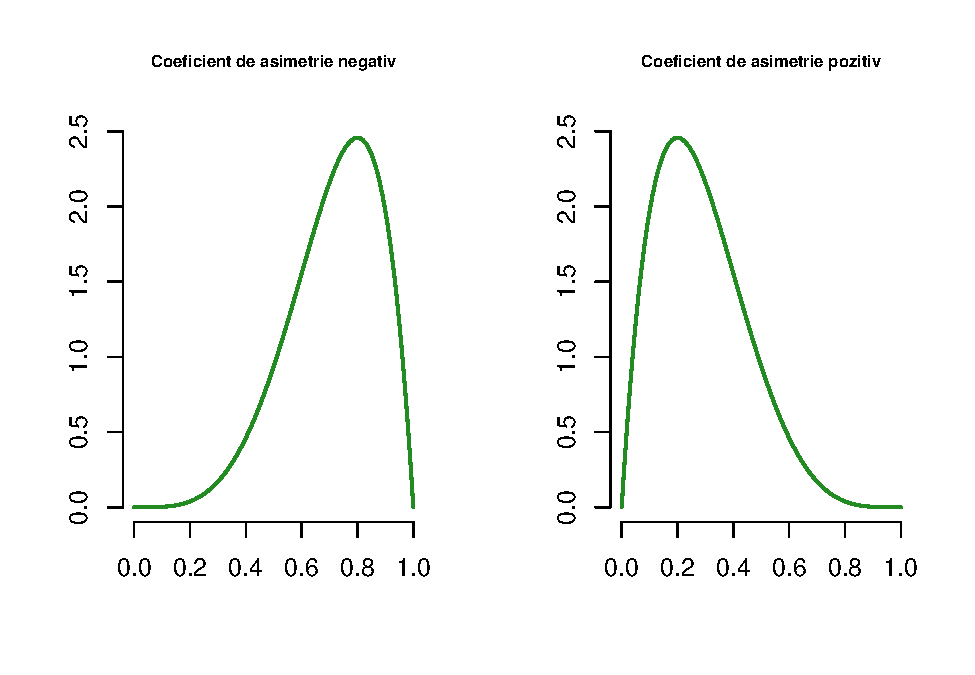
\includegraphics[width=0.8\linewidth]{Lab_4_files/figure-latex/unnamed-chunk-2-1} \end{center}

Coeficientul de asimetrie pentru un eșantion \(X_1, X_2, \ldots, X_n\)
este

\[
  b_1 = \frac{\frac{1}{n}\sum_{i = 1}^{n} (X_i - \bar{X}_n)^3}{\left(\frac{1}{n}\sum_{i = 1}^{n} (X_i - \bar{X}_n)^2\right)^{\frac{3}{2}}}.
\]

Coeficientul de aplatizare (\emph{kurtosis}) măsoară dacă datele au
coadă mai lungă sau mai scurtă în raport cu repartiția normală. Fiind
dată o variabilă aleatoare \(X\) cu \(\mathbb{E}[X^4]<\infty\),
\(\mathbb{E}[X]=\mu\) și \(Var(X)=\sigma^2>0\) coeficientul de
aplatizare este definit prin relația

\[
  \gamma_2(X) = \mathbb{E}\left[\frac{(X-\mu)^4}{\sigma^4}\right] - 3.
\]

Pentru o variabilă aleatoare repartizată normal,
\(Z\sim \mathcal{N}(\mu, \sigma^2)\), avem că \(\gamma_2(Z) = 0\).

Coeficientul de aplatizare pentru un eșantion \(X_1, X_2, \ldots, X_n\)
este

\[
  b_2 = \frac{\frac{1}{n}\sum_{i = 1}^{n} (X_i - \bar{X}_n)^4}{\left(\frac{1}{n}\sum_{i = 1}^{n} (X_i - \bar{X}_n)^2\right)^{2}} - 3.
\] Articolul (Gill 1998) prezintă diferite metode de calcul pentru
coeficientul de aplatizare și cel de asimetrie într-un eșantion.

\begin{rmdexercise}
Construiți în R două funcții, \texttt{skewness\_coef()} și
\texttt{kurtosis\_coef()}, care să permită calculul coeficientului de
asimetrie și respectiv a coeficientului de aplatizare pentru un eșantion
dat.
\end{rmdexercise}

Deplasarea față de valoarea \(0\), atât pentru coeficientul de asimetrie
cât și pentru cel de aplatizare indică o deplasare față de repartiția
normală. Pentru a decide dacă o anumită deplasare față de \(0\) este
mare sau mică se poate folosi un studiu de simulare. De exemplu,
coeficientul de asimetrie calculat pentru greutatea la naștere a celor
189 de copii din setul de date \texttt{birthwt} (din pachetul
\texttt{MASS}) este -0.207 iar coeficientul de aplatizare este -0.113.
Pentru a vedea dacă -0.207 și respectiv dacă -0.113 sunt valori tipice
pentru coeficientul de asimetrie și respectiv de aplatizare dintr-un
eșantion de 189 de observații dintr-o populație normală, repetăm
următorul proces de un număr mare de ori (de exemplu \(10000\)): generăm
aletor 189 de observații dintr-o repartiție normală și calculăm cei doi
coeficienți.

\begin{Shaded}
\begin{Highlighting}[]
\KeywordTok{library}\NormalTok{(MASS)}
\NormalTok{weight =}\StringTok{ }\NormalTok{birthwt}\OperatorTok{$}\NormalTok{bwt}

\NormalTok{n_wt =}\StringTok{ }\KeywordTok{length}\NormalTok{(weight)}
\NormalTok{m_wt =}\StringTok{ }\KeywordTok{mean}\NormalTok{(weight)}
\NormalTok{sd_wt =}\StringTok{ }\KeywordTok{sd}\NormalTok{(weight)}

\NormalTok{skew_bwt =}\StringTok{ }\KeywordTok{skewness_coef}\NormalTok{(weight)}
\NormalTok{kurt_bwt =}\StringTok{ }\KeywordTok{kurtosis_coef}\NormalTok{(weight)}

\CommentTok{# functia de simulare}
\NormalTok{skew_kurt_sim =}\StringTok{ }\ControlFlowTok{function}\NormalTok{(}\DataTypeTok{fun =} \ControlFlowTok{function}\NormalTok{(n) }\KeywordTok{rnorm}\NormalTok{(n), }\DataTypeTok{n =} \DecValTok{100}\NormalTok{)\{}
\NormalTok{  x =}\StringTok{ }\KeywordTok{fun}\NormalTok{(n)}
\NormalTok{  kurt =}\StringTok{ }\KeywordTok{kurtosis_coef}\NormalTok{(x)}
\NormalTok{  skew =}\StringTok{ }\KeywordTok{skewness_coef}\NormalTok{(x)}
  
  \KeywordTok{return}\NormalTok{(}\KeywordTok{c}\NormalTok{(}\DataTypeTok{kurtosis =}\NormalTok{ kurt, }\DataTypeTok{skewness =}\NormalTok{ skew))}
\NormalTok{\}}

\CommentTok{# replicam de 10000 de ori procesul }
\NormalTok{out1 <-}\StringTok{ }\KeywordTok{replicate}\NormalTok{(}\DecValTok{10000}\NormalTok{, }
         \KeywordTok{skew_kurt_sim}\NormalTok{(}\DataTypeTok{fun =} \ControlFlowTok{function}\NormalTok{(n) }\KeywordTok{rnorm}\NormalTok{(n), }
                       \DataTypeTok{n =}\NormalTok{ n_wt))}
\end{Highlighting}
\end{Shaded}

Figurile de mai jos reprezintă histogramele a \(10000\) de valori ale
coeficientului de asimetrie și respectiv de aplatizare, calculate pentru
\(10000\) de eșantioane de talie 189 dintr-o repartiție normală
standard.

\begin{center}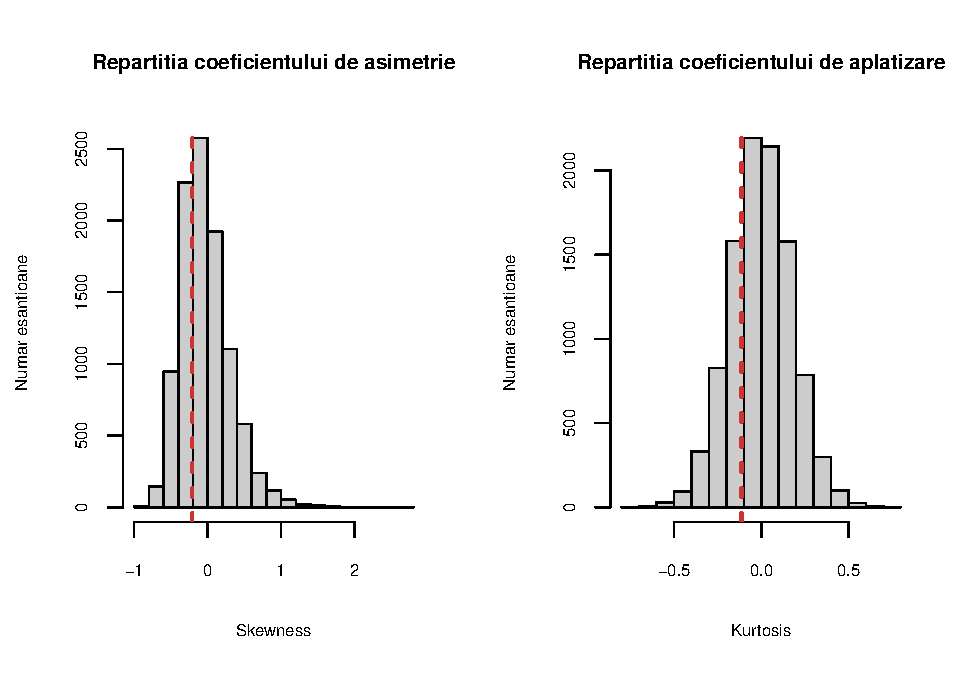
\includegraphics[width=0.8\linewidth]{Lab_4_files/figure-latex/unnamed-chunk-6-1} \end{center}

\section{Metoda grafică: Q-Q plot}\label{metoda-grafica-q-q-plot}

Graficul cuantilă-cuantilă (\emph{quantile-quantile plot} sau \emph{q-q
plot} pe scurt) este o metodă grafică introdusă în (Wilk and
Gnanadesikan 1968) și folosită pentru a determina dacă două eșantioane
provin din populații cu repartiție comună. Un \emph{q-q plot} ilustrează
grafic cuantilele empirice ale primului eșantion față de cuantilele
empirice (sau teoretice) ale celui de-al doilea eșantion.

Fiind date două eșantioane, \(X_1,X_2,\ldots,X_n\sim F\) și respectiv
\(Y_1, Y_2, \ldots, Y_m\sim G\), fie
\(\hat{x}_p(n) = \hat{F}_n^{-1}(p)\) și
\(\hat{y}_p(m) = \hat{G}_m^{-1}(p)\) cuantilele empirice de ordin \(p\)
asociate celor două eșantioane. Metoda \emph{q-q plot} implică trasarea
pe același grafic al punctelor de coordonate
\((\hat{x}_p(n), \hat{y}_p(m))\) pentru diverse valori ale lui
\(p\in(0,1)\). După cum am văzut în
\href{https://alexamarioarei.github.io/Teaching/2017-2018/Instrumente\%20Statistice\%20web\%20page/labs/Lab_3.html}{Laboratorul
3}, cunatila empirică de ordin \(p\) coincide cu una dintre statisticile
de ordine
\(\hat{x}_p = X_{(i)} \iff \hat{x}_p = X_{(\lceil np \rceil)}\) (deci
\(X_{(k)}\) este cuantila de ordin \(\frac{k}{n}\)) și prin urmare putem
considera că

\[
    p\in \left\{\begin{array}{ll}
      \left\{\frac{i}{n}\,|\,1\leq i\leq n\right\}, & n\leq m\\
      \left\{\frac{i}{m}\,|\,1\leq i\leq m\right\}, & n\geq m.
    \end{array}\right.
  \] În practică, pentru a avea \(p<1\) vom considera că \(X_{(k)}\)
este cuantila de ordin \(\frac{k}{n+1}\) (unii autori consideră că
\(X_{(k)}\) este cuantila de ordin \(\frac{k-0.5}{n}\) sau încă de ordin
\(\frac{k-3/8}{n+1/4}\)), astfel

\[
    p\in \left\{\begin{array}{ll}
      \left\{\frac{i}{n+1}\,|\,1\leq i\leq n\right\}, & n\leq m\\
      \left\{\frac{i}{m+1}\,|\,1\leq i\leq m\right\}, & n\geq m.
    \end{array}\right.
  \]

În R putem folosi funcția \texttt{qqplot()} pentru a trasa graficul
cuantilă-cuantilă (tastați \texttt{?qqplot} pentru a vedea documentația
acestei funcții).

\begin{rmdexercise}
Construiți în R o funcție \texttt{qqgraf()} care să traseze graficul
cuantilă-cuantilă pentru două eșantioane.
\end{rmdexercise}

Observăm că dacă cele două eșantioane ar proveni de la aceeași populație
(\(F = G\)) atunci punctele ar fi aliniate aproximativ pe o dreaptă
(prima bisectoare \(y=x\)).

\begin{Shaded}
\begin{Highlighting}[]
\NormalTok{x =}\StringTok{ }\KeywordTok{rnorm}\NormalTok{(}\DecValTok{100}\NormalTok{)}
\NormalTok{y=}\StringTok{ }\KeywordTok{rnorm}\NormalTok{(}\DecValTok{150}\NormalTok{)}

\KeywordTok{qqgraf}\NormalTok{(x, y)}
\end{Highlighting}
\end{Shaded}

\begin{center}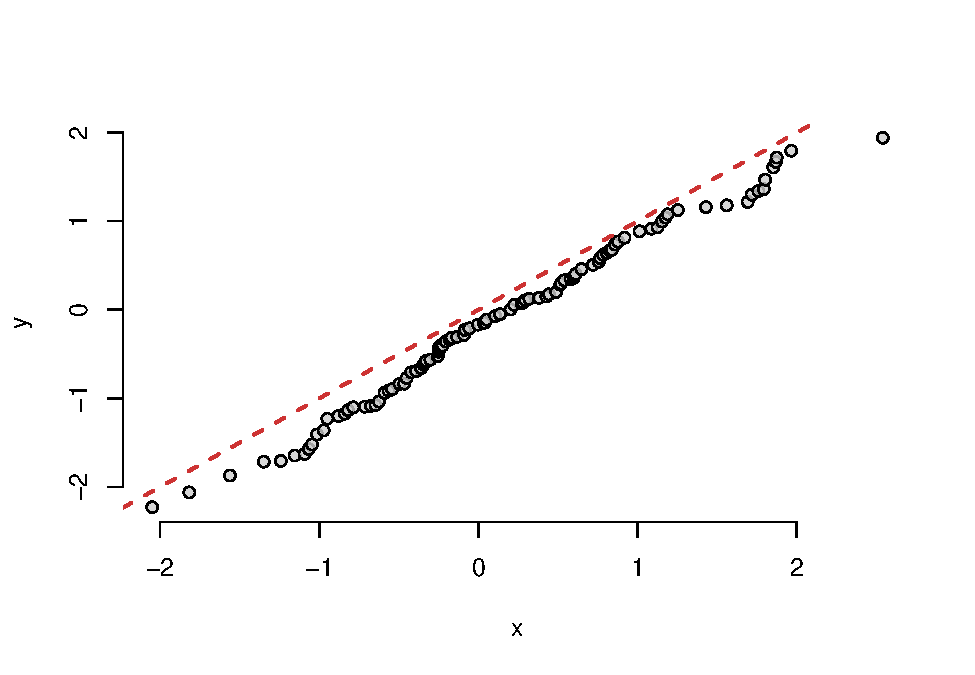
\includegraphics[width=0.8\linewidth]{Lab_4_files/figure-latex/unnamed-chunk-9-1} \end{center}

O deviere de la prima bisectoare indică o diferență între formele celor
două distribuții din care au provenit datele. Atunci când cele două
repartiții au aceeași formă dar au medii și respectiv abateri standard
diferite atunci graficul rămâne liniar numai că ordonata la origine și
panta dreptei nu vor mai fi \(0\) și respectiv \(1\). O ordonată la
origine diferită de \(0\) arată o translatare în repartiții (schimbare
de locație) iar o pantă neunitară indică o schimbare de scală.

\begin{Shaded}
\begin{Highlighting}[]
\KeywordTok{par}\NormalTok{(}\DataTypeTok{mfrow =} \KeywordTok{c}\NormalTok{(}\DecValTok{1}\NormalTok{,}\DecValTok{2}\NormalTok{))}

\NormalTok{x =}\StringTok{ }\KeywordTok{rnorm}\NormalTok{(}\DecValTok{200}\NormalTok{, }\DecValTok{2}\NormalTok{, }\DecValTok{1}\NormalTok{)}
\NormalTok{y=}\StringTok{ }\KeywordTok{rnorm}\NormalTok{(}\DecValTok{150}\NormalTok{)}
\KeywordTok{qqgraf}\NormalTok{(x, y, }\DataTypeTok{main =} \StringTok{"Translatare"}\NormalTok{)}
\KeywordTok{abline}\NormalTok{(}\DataTypeTok{a =} \OperatorTok{-}\DecValTok{2}\NormalTok{, }\DataTypeTok{b =} \DecValTok{1}\NormalTok{, }
       \DataTypeTok{col =} \StringTok{"grey80"}\NormalTok{, }
       \DataTypeTok{lty =} \DecValTok{2}\NormalTok{, }\DataTypeTok{lwd =} \DecValTok{2}\NormalTok{)}

\NormalTok{x =}\StringTok{ }\KeywordTok{rnorm}\NormalTok{(}\DecValTok{200}\NormalTok{, }\DecValTok{0}\NormalTok{, }\DecValTok{2}\NormalTok{)}
\NormalTok{y=}\StringTok{ }\KeywordTok{rnorm}\NormalTok{(}\DecValTok{150}\NormalTok{)}
\KeywordTok{qqgraf}\NormalTok{(x, y, }\DataTypeTok{main =} \StringTok{"Scalare"}\NormalTok{)}
\KeywordTok{abline}\NormalTok{(}\DataTypeTok{a =} \DecValTok{0}\NormalTok{, }\DataTypeTok{b =} \DecValTok{1}\OperatorTok{/}\DecValTok{2}\NormalTok{, }
       \DataTypeTok{col =} \StringTok{"grey80"}\NormalTok{,}
       \DataTypeTok{lty =} \DecValTok{2}\NormalTok{, }\DataTypeTok{lwd =} \DecValTok{2}\NormalTok{)}
\end{Highlighting}
\end{Shaded}

\begin{center}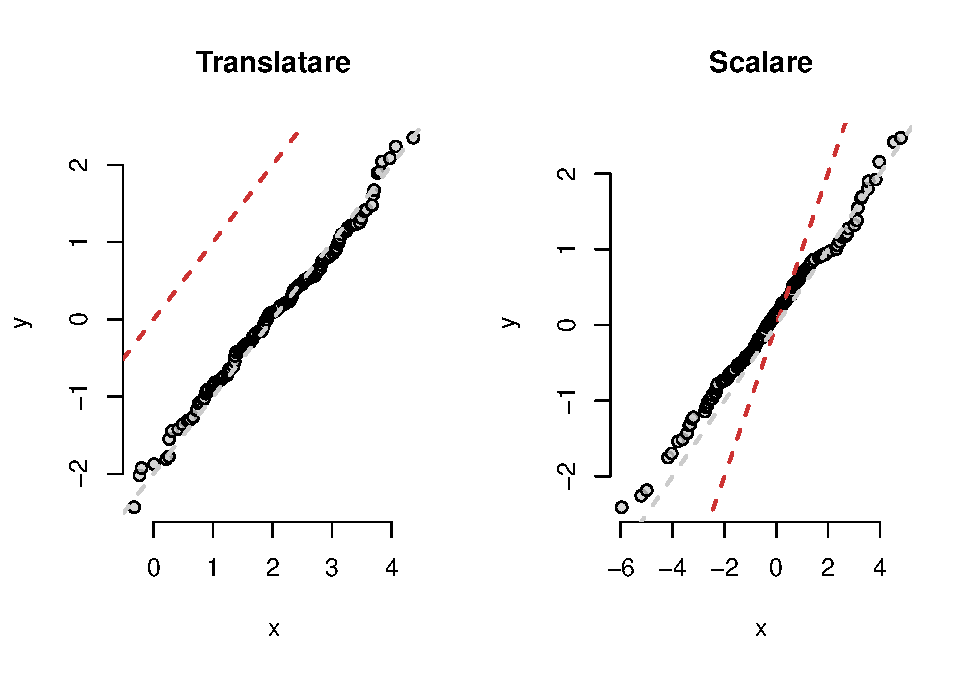
\includegraphics[width=0.8\linewidth]{Lab_4_files/figure-latex/unnamed-chunk-10-1} \end{center}

Graficul cuantilă-cuantilă poate fi folosit și pentru a verifica dacă un
eșantion provine dintr-o repartiție specificată, astfel dat fiind
\((X_1, X_2, \ldots, X_n)(\omega) = (x_1, x_2, \ldots, x_n)\) un
eșantion de talie \(n\) vrem să verificăm dacă acesta provine dintr-o
populație (specificată) \(F\). Dacă \(\hat{x}_p(n)\) este cuantila
empirică de ordin \(p\) și \(x_p = F^{-1}(p)\) este cuantila teoretică
de ordin \(p\) asociată lui \(F\), atunci graficul cuantilă-cuantilă
este determinat de punctele \(\left(x_p,\hat{x}_p(n)\right)\),
\(p\in(0,1)\). Folosind alegerea lui \(p\) de mai sus (care evită
singularitățile \(F^{-1}(1) = \infty\)) și ținând cont că
\(\hat{x}_{\frac{i}{n+1}}(n) = X_{(i)}\) avem că graficul
cuantilă-cuantilă este determinat de mulțimea de puncte

\[
  \mathcal{G} = \left\{\left(F^{-1}\left(\frac{i}{n+1}\right), X_{(i)}\right)\,|\, 1\leq i\leq n\right\}. 
\]

Pentru a verifica dacă datele provin dintr-o repartiție normală este
suficient să alegem \(F = \Phi\), cu \(\Phi(x)\) funcția de repartiție a
normalei standard (acest grafic se mai numește și \emph{normal
probability plot} sau \emph{normal-quantile plot}). Dacă punctele se
află (aproximativ) pe o dreaptă atunci putem spune că datele provin
dintr-o repartiție (aproximativ) normală. Deplasarea față de normalitate
este indicată prin deplasarea față de o dreaptă. Un grafic în formă de
\emph{U} arată că repartiția este asimetrică iar un grafic în formă de
\emph{S} ne spune că avem diferențe între coada repartiției normale și
cea care a generat setul de date.

În R putem trasa graficul cuantilă-cuantilă pentru o populașie normală
cu ajutorul funcției \texttt{qqnorm()} iar dreapta de referință cu
ajutorul funcției \texttt{qqline()}. Pentru mai multe detalii privind
aceste funcții tastați \texttt{?qqnorm} și \texttt{?qqline}.

\begin{rmdexercise}
Construiți în R o funcție \texttt{qq\_norm()} care să traseze graficul
cuantilă-cuantilă (\emph{normal-quantile plot}) pentru a verifica dacă
un eșantion provine dintr-o populație normală.
\end{rmdexercise}

\begin{Shaded}
\begin{Highlighting}[]
\KeywordTok{par}\NormalTok{(}\DataTypeTok{mfrow =} \KeywordTok{c}\NormalTok{(}\DecValTok{2}\NormalTok{,}\DecValTok{2}\NormalTok{))}
\NormalTok{n =}\StringTok{ }\DecValTok{250}
\CommentTok{# coada scurta }
\NormalTok{x_st =}\StringTok{ }\KeywordTok{runif}\NormalTok{(n, }\DataTypeTok{min=}\DecValTok{0}\NormalTok{, }\DataTypeTok{max=}\DecValTok{2}\NormalTok{)}
\KeywordTok{qq_norm}\NormalTok{(x_st, }\DataTypeTok{main =} \StringTok{"Coada scurta"}\NormalTok{)}

\CommentTok{# coada lunga }
\NormalTok{x_ht =}\StringTok{ }\KeywordTok{rcauchy}\NormalTok{(n, }\DataTypeTok{location=}\DecValTok{0}\NormalTok{, }\DataTypeTok{scale=}\DecValTok{1}\NormalTok{)}
\KeywordTok{qq_norm}\NormalTok{(x_ht, }\DataTypeTok{main =} \StringTok{"Coada lunga"}\NormalTok{)}

\CommentTok{# asimetrica spre stanga }
\NormalTok{x_sn =}\StringTok{ }\KeywordTok{rbeta}\NormalTok{(n, }\DecValTok{2}\NormalTok{, }\FloatTok{0.5}\NormalTok{, }\DataTypeTok{ncp =} \DecValTok{2}\NormalTok{)}
\KeywordTok{qq_norm}\NormalTok{(x_sn, }\DataTypeTok{main =} \StringTok{"Asimetrica spre stanga"}\NormalTok{)}

\CommentTok{# asimetrica spre dreapta }
\NormalTok{x_sp =}\StringTok{ }\KeywordTok{rexp}\NormalTok{(n, }\DecValTok{2}\NormalTok{)}
\KeywordTok{qq_norm}\NormalTok{(x_sp, }\DataTypeTok{main =} \StringTok{"Asimetrica spre dreapta"}\NormalTok{)}
\end{Highlighting}
\end{Shaded}

\begin{center}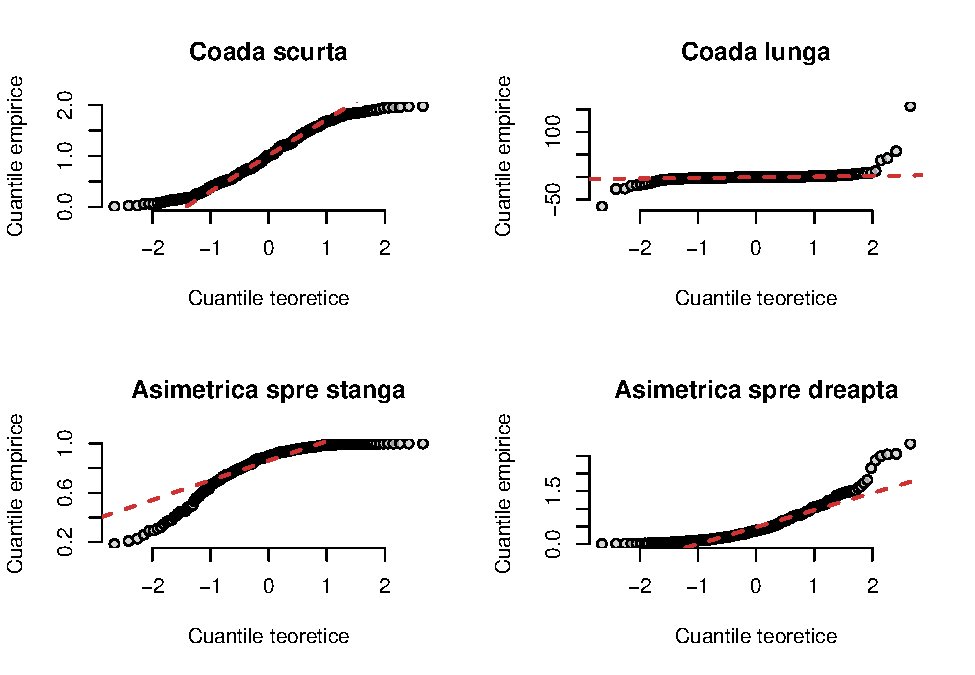
\includegraphics[width=0.8\linewidth]{Lab_4_files/figure-latex/unnamed-chunk-13-1} \end{center}

\begin{rmdexercise}
Considerați setul de date \texttt{birthwt} din pachetul \texttt{MASS}.
Trasați histograma greutății la naștere a copiilor (variabila
\texttt{bwt}) și graficul cuantilă-cuantilă pentru o populație normală.
Comparați grafic dacă repartiția greutății copiilor la naștere diferă în
funcție de statutul de fumător al mamei.
\end{rmdexercise}

\begin{Shaded}
\begin{Highlighting}[]
\KeywordTok{par}\NormalTok{(}\DataTypeTok{mfrow =} \KeywordTok{c}\NormalTok{(}\DecValTok{1}\NormalTok{,}\DecValTok{2}\NormalTok{), }
    \DataTypeTok{cex.main =} \FloatTok{0.8}\NormalTok{,}
    \DataTypeTok{cex.axis =} \FloatTok{0.7}\NormalTok{,}
    \DataTypeTok{cex.lab =} \FloatTok{0.7}\NormalTok{)}

\KeywordTok{hist}\NormalTok{(birthwt}\OperatorTok{$}\NormalTok{bwt, }
     \DataTypeTok{probability =} \OtherTok{TRUE}\NormalTok{, }
     \DataTypeTok{col =} \StringTok{"grey80"}\NormalTok{,}
     \DataTypeTok{main =} \StringTok{"Repartitia greutatii"}\NormalTok{,}
     \DataTypeTok{xlab =} \StringTok{"Greutatea la nastere"}\NormalTok{,}
     \DataTypeTok{ylab =} \StringTok{"Densitate"}\NormalTok{)}

\NormalTok{t =}\StringTok{ }\KeywordTok{seq}\NormalTok{(}\KeywordTok{min}\NormalTok{(birthwt}\OperatorTok{$}\NormalTok{bwt), }\KeywordTok{max}\NormalTok{(birthwt}\OperatorTok{$}\NormalTok{bwt), }
        \DataTypeTok{length.out =} \DecValTok{100}\NormalTok{)}
\NormalTok{x =}\StringTok{ }\KeywordTok{dnorm}\NormalTok{(t, }\KeywordTok{mean}\NormalTok{(birthwt}\OperatorTok{$}\NormalTok{bwt), }\KeywordTok{sd}\NormalTok{(birthwt}\OperatorTok{$}\NormalTok{bwt))}

\KeywordTok{lines}\NormalTok{(t, x, }\DataTypeTok{lwd =} \DecValTok{2}\NormalTok{, }\DataTypeTok{lty =} \DecValTok{2}\NormalTok{,}
      \DataTypeTok{col =} \StringTok{"brown3"}\NormalTok{)}

\KeywordTok{qq_norm}\NormalTok{(birthwt}\OperatorTok{$}\NormalTok{bwt, }
        \DataTypeTok{main =} \StringTok{"Graficul cuantila-cuantila"}\NormalTok{)}
\end{Highlighting}
\end{Shaded}

\begin{center}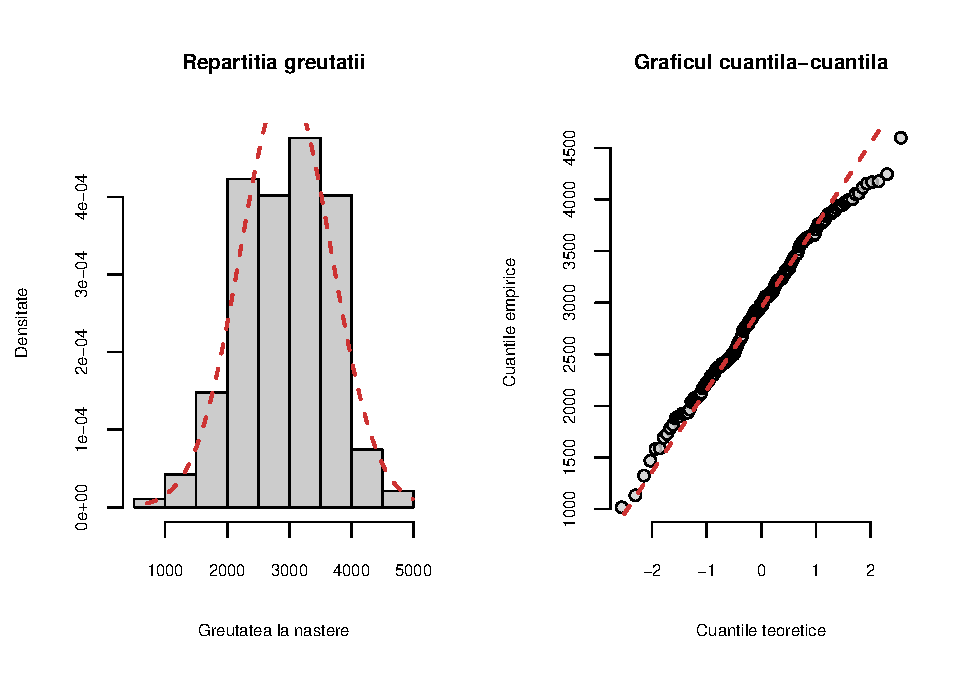
\includegraphics[width=0.8\linewidth]{Lab_4_files/figure-latex/unnamed-chunk-15-1} \end{center}

\begin{Shaded}
\begin{Highlighting}[]
\KeywordTok{par}\NormalTok{(}\DataTypeTok{mfrow =} \KeywordTok{c}\NormalTok{(}\DecValTok{2}\NormalTok{,}\DecValTok{2}\NormalTok{),}
     \DataTypeTok{cex.main =} \FloatTok{0.8}\NormalTok{,}
     \DataTypeTok{cex.axis =} \FloatTok{0.7}\NormalTok{,}
     \DataTypeTok{cex.lab =} \FloatTok{0.7}\NormalTok{)}

\NormalTok{bwt_nf =}\StringTok{ }\NormalTok{birthwt}\OperatorTok{$}\NormalTok{bwt[birthwt}\OperatorTok{$}\NormalTok{smoke }\OperatorTok{==}\StringTok{ }\DecValTok{0}\NormalTok{]}
\NormalTok{bwt_f =}\StringTok{ }\NormalTok{birthwt}\OperatorTok{$}\NormalTok{bwt[birthwt}\OperatorTok{$}\NormalTok{smoke }\OperatorTok{==}\StringTok{ }\DecValTok{1}\NormalTok{]}
\NormalTok{bwt =}\StringTok{ }\NormalTok{birthwt}\OperatorTok{$}\NormalTok{bwt}

\CommentTok{# nefumatoare}
\KeywordTok{hist}\NormalTok{(bwt_nf, }\DataTypeTok{proba =} \OtherTok{TRUE}\NormalTok{,}
      \DataTypeTok{breaks=}\DecValTok{25}\NormalTok{,}
      \DataTypeTok{col =} \KeywordTok{grey}\NormalTok{(}\FloatTok{0.8}\NormalTok{),}
      \DataTypeTok{main =} \StringTok{"Greutatea copiilor}\CharTok{\textbackslash{}n}\StringTok{ (mame nefumatoare)"}\NormalTok{,}
      \DataTypeTok{xlab =} \StringTok{"Greutatea la nastere"}\NormalTok{,}
      \DataTypeTok{ylab =} \StringTok{"densitatea"}\NormalTok{,}
      \DataTypeTok{ylim =} \KeywordTok{c}\NormalTok{(}\DecValTok{0}\NormalTok{, }\FloatTok{6e-4}\NormalTok{))}

\NormalTok{t_nf =}\StringTok{ }\KeywordTok{seq}\NormalTok{(}\KeywordTok{min}\NormalTok{(bwt_nf), }\KeywordTok{max}\NormalTok{(bwt_nf), }
        \DataTypeTok{length.out =} \DecValTok{100}\NormalTok{)}

\NormalTok{x_nf =}\StringTok{ }\KeywordTok{dnorm}\NormalTok{(t_nf, }\KeywordTok{mean}\NormalTok{(bwt_nf), }\KeywordTok{sd}\NormalTok{(bwt_nf))}

\KeywordTok{lines}\NormalTok{(t_nf, x_nf, }\DataTypeTok{col =} \StringTok{"brown3"}\NormalTok{,}
      \DataTypeTok{lty =} \DecValTok{2}\NormalTok{, }\DataTypeTok{lwd =} \DecValTok{2}\NormalTok{)}

\KeywordTok{qq_norm}\NormalTok{(bwt_nf,}
        \DataTypeTok{main =} \StringTok{"Graficul cuantila-cuantila"}\NormalTok{)}

\CommentTok{# fumatoare}
\KeywordTok{hist}\NormalTok{(bwt_f, }\DataTypeTok{proba =} \OtherTok{TRUE}\NormalTok{,}
      \DataTypeTok{breaks=}\DecValTok{25}\NormalTok{,}
      \DataTypeTok{col =} \KeywordTok{grey}\NormalTok{(}\FloatTok{0.8}\NormalTok{),}
      \DataTypeTok{main =} \StringTok{"Greutatea copiilor}\CharTok{\textbackslash{}n}\StringTok{ (mame fumatoare)"}\NormalTok{,}
      \DataTypeTok{xlab =} \StringTok{"Greutatea la nastere"}\NormalTok{,}
      \DataTypeTok{ylab =} \StringTok{"densitatea"}\NormalTok{,}
      \DataTypeTok{ylim =} \KeywordTok{c}\NormalTok{(}\DecValTok{0}\NormalTok{, }\FloatTok{6e-4}\NormalTok{))}

\NormalTok{t_f =}\StringTok{ }\KeywordTok{seq}\NormalTok{(}\KeywordTok{min}\NormalTok{(bwt_nf), }\KeywordTok{max}\NormalTok{(bwt_nf), }
        \DataTypeTok{length.out =} \DecValTok{100}\NormalTok{)}

\NormalTok{x_f =}\StringTok{ }\KeywordTok{dnorm}\NormalTok{(t_f, }\KeywordTok{mean}\NormalTok{(bwt_f), }\KeywordTok{sd}\NormalTok{(bwt_f))}

\KeywordTok{lines}\NormalTok{(t_f, x_f, }\DataTypeTok{col =} \StringTok{"brown3"}\NormalTok{,}
      \DataTypeTok{lty =} \DecValTok{2}\NormalTok{, }\DataTypeTok{lwd =} \DecValTok{2}\NormalTok{)}

\KeywordTok{qq_norm}\NormalTok{(bwt_f,}
        \DataTypeTok{main =} \StringTok{"Graficul cuantila-cuantila"}\NormalTok{)}
\end{Highlighting}
\end{Shaded}

\begin{center}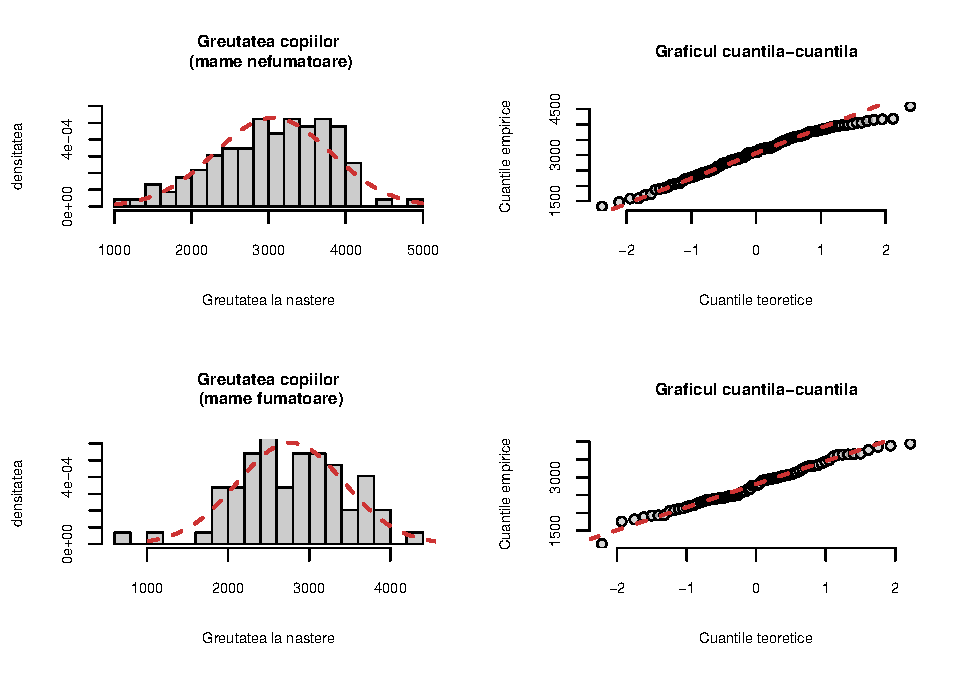
\includegraphics[width=0.8\linewidth]{Lab_4_files/figure-latex/unnamed-chunk-16-1} \end{center}

Ce se întâmplă atunci când avem o mixtură de repartiții? Următoarea
funcție permite generarea unui eșantion dintr-o mixtură de două
repartiții normale:

\[
  f(x) = p\frac{1}{\sqrt{2\pi\sigma_1^2}}e^{-\frac{1}{2}\left(\frac{x-\mu_1}{\sigma_1}\right)^2} + (1-p)\frac{1}{\sqrt{2\pi\sigma_2^2}}e^{-\frac{1}{2}\left(\frac{x-\mu_2}{\sigma_2}\right)^2}, \; p\in (0,1)
\]

\begin{Shaded}
\begin{Highlighting}[]
\NormalTok{mix_norm_sim =}\StringTok{ }\ControlFlowTok{function}\NormalTok{(}\DataTypeTok{n =} \DecValTok{100}\NormalTok{, }\DataTypeTok{p =} \FloatTok{0.5}\NormalTok{, }\DataTypeTok{m1 =} \OperatorTok{-}\DecValTok{1}\NormalTok{, }\DataTypeTok{sd1 =} \DecValTok{1}\NormalTok{, }\DataTypeTok{m2 =} \DecValTok{2}\NormalTok{, }\DataTypeTok{sd2 =} \DecValTok{2}\NormalTok{)\{}
\NormalTok{  n1 =}\StringTok{ }\KeywordTok{rbinom}\NormalTok{(}\DecValTok{1}\NormalTok{,n,p)}
\NormalTok{  x1 =}\StringTok{ }\KeywordTok{rnorm}\NormalTok{(n1, }\DataTypeTok{m =}\NormalTok{ m1, }\DataTypeTok{sd =}\NormalTok{ sd1)}
\NormalTok{  x2 =}\StringTok{ }\KeywordTok{rnorm}\NormalTok{(n}\OperatorTok{-}\NormalTok{n1, }\DataTypeTok{m =}\NormalTok{ m2, }\DataTypeTok{sd =}\NormalTok{ sd2)}
  \KeywordTok{c}\NormalTok{(x1, x2)}
\NormalTok{\}}
\end{Highlighting}
\end{Shaded}

Ilustrăm grafic metoda cuantilă-cuantilă pentru diferite scenarii:

\begin{Shaded}
\begin{Highlighting}[]
\KeywordTok{par}\NormalTok{(}\DataTypeTok{mfrow=}\KeywordTok{c}\NormalTok{(}\DecValTok{2}\NormalTok{,}\DecValTok{2}\NormalTok{),}
     \DataTypeTok{cex.main =} \FloatTok{0.8}\NormalTok{,}
     \DataTypeTok{cex.axis =} \FloatTok{0.7}\NormalTok{,}
     \DataTypeTok{cex.lab =} \FloatTok{0.7}\NormalTok{)}
\CommentTok{#----------}
\NormalTok{w0 =}\StringTok{ }\KeywordTok{mix_norm_sim}\NormalTok{(}\DecValTok{1000}\NormalTok{,}\FloatTok{0.25}\NormalTok{,}\OperatorTok{-}\DecValTok{20}\NormalTok{,}\DecValTok{10}\NormalTok{,}\DecValTok{20}\NormalTok{,}\DecValTok{10}\NormalTok{)}
\KeywordTok{hist}\NormalTok{(w0, }\DataTypeTok{col =} \KeywordTok{grey}\NormalTok{(}\FloatTok{0.8}\NormalTok{),}
     \DataTypeTok{probability =} \OtherTok{TRUE}\NormalTok{,}
     \DataTypeTok{main =} \StringTok{"Scenariul 1"}\NormalTok{, }
     \DataTypeTok{xlab =} \StringTok{"Observatii"}\NormalTok{, }
     \DataTypeTok{ylab =} \StringTok{"Densitatea"}\NormalTok{)}
\KeywordTok{qq_norm}\NormalTok{(w0, }\DataTypeTok{main =} \StringTok{"Q-Q plot - Scenariul 1"}\NormalTok{)}
\CommentTok{#----------}
\NormalTok{w1 =}\StringTok{ }\KeywordTok{mix_norm_sim}\NormalTok{(}\DecValTok{1000}\NormalTok{,}\FloatTok{0.5}\NormalTok{,}\DecValTok{0}\NormalTok{,}\DecValTok{1}\NormalTok{,}\DecValTok{5}\NormalTok{,}\DecValTok{1}\NormalTok{)}
\KeywordTok{hist}\NormalTok{(w1, }\DataTypeTok{col =} \KeywordTok{grey}\NormalTok{(}\FloatTok{0.8}\NormalTok{),}
     \DataTypeTok{probability =} \OtherTok{TRUE}\NormalTok{,}
     \DataTypeTok{main =} \StringTok{"Scenariul 2"}\NormalTok{, }
     \DataTypeTok{xlab =} \StringTok{"Observatii"}\NormalTok{, }
     \DataTypeTok{ylab =} \StringTok{"Densitatea"}\NormalTok{)}
\KeywordTok{qq_norm}\NormalTok{(w1, }\DataTypeTok{main =} \StringTok{"Q-Q plot - Scenariul 2"}\NormalTok{)}
\end{Highlighting}
\end{Shaded}

\begin{center}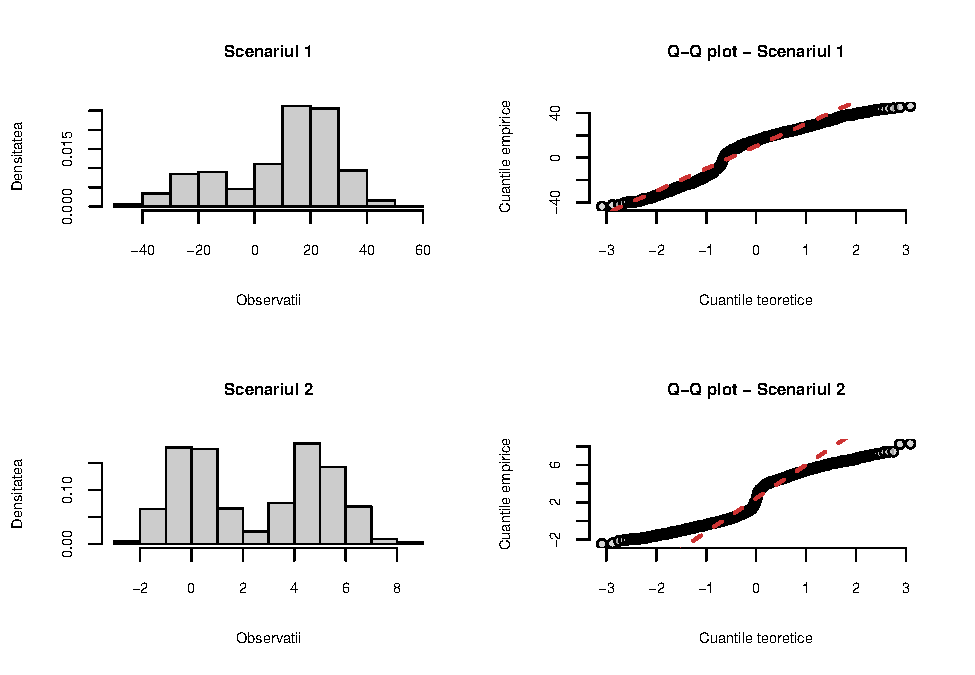
\includegraphics[width=0.8\linewidth]{Lab_4_files/figure-latex/unnamed-chunk-18-1} \end{center}

\section{Teste statistice}\label{teste-statistice}

Chiar dacă metodele grafice (e.g.~histograma sau graficul
cuantilă-cuantilă) pot conduce la ipoteza de normalitate, acestea nu
sunt suficiente. Pentru a putea folosi modelul de normalitate a datelor
este necesar să efectuăm un test statistic care să respingă sau să nu
respingă ipoteza de normalitate a populației din care a provenit
eșantionul. În cele ce urmează vom prezenta mai multe teste statistice
folosite pentru testarea ipotezei de normalitate:

\[
\begin{array}{ll}
  H_0:\,\text{eșantionul nu este semnificativ diferit de o populație normală}\\
  H_1:\,\text{eșantionul este semnificativ diferit de o populație normală}
\end{array}
\]

Literatura de specialitate este foarte vastă în ceea ce privește testele
statistice folosite pentru testarea ipotezei de normalitate, de exemplu
articolul (Romão 2010) compară peste 30 astfel de teste (și cartea
(Thode 2002) prezintă o colecție de astfel de teste).

\subsection{Testul lui Jarque-Bera}\label{testul-lui-jarque-bera}

Plecând de la coeficientul de asimetrie și coeficientul de aplatizare a
unui eșantion, C. Jarque și A. Bera au propus în (Jarque and Bera 1987)
următoarea statistică de test pentru testarea ipotezei de normalitate a
datelor

\[
  JB = \frac{n}{6}\left(b_1^2 + \frac{b_2^2}{4}\right).
\]

Autorii au arătat că dacă datele sunt normale și \(n\) este suficient de
mare atunci \(JB\overset{d}{\to}\chi^2(2)\).

\begin{rmdexercise}
Construiți în R o funcție \texttt{JBtest()} care să implementeze testul
Jarque-Bera. Aplicați testul pentru o serie de exemple.
\end{rmdexercise}

\begin{Shaded}
\begin{Highlighting}[]
\CommentTok{# pentru esantion normal }
\NormalTok{x =}\StringTok{ }\KeywordTok{rnorm}\NormalTok{(}\DecValTok{1000}\NormalTok{)}
\KeywordTok{JBtest}\NormalTok{(x)}

\NormalTok{    Jarque Bera Test}

\NormalTok{data}\OperatorTok{:}\StringTok{  }\NormalTok{x}
\NormalTok{=}\StringTok{ }\FloatTok{2.0635}\NormalTok{, df =}\StringTok{ }\DecValTok{2}\NormalTok{, p}\OperatorTok{-}\NormalTok{value =}\StringTok{ }\FloatTok{0.3564}

\CommentTok{# pentru esantion exponential  }
\NormalTok{x =}\StringTok{ }\KeywordTok{rexp}\NormalTok{(}\DecValTok{100}\NormalTok{, }\FloatTok{0.2}\NormalTok{)}
\KeywordTok{JBtest}\NormalTok{(x)}

\NormalTok{    Jarque Bera Test}

\NormalTok{data}\OperatorTok{:}\StringTok{  }\NormalTok{x}
\NormalTok{=}\StringTok{ }\FloatTok{91.352}\NormalTok{, df =}\StringTok{ }\DecValTok{2}\NormalTok{, p}\OperatorTok{-}\NormalTok{value }\OperatorTok{<}\StringTok{ }\FloatTok{2.2e-16}
\end{Highlighting}
\end{Shaded}

\subsection{Testul lui Shapiro-Wilk și varianta lui
Shapiro-Francia}\label{testul-lui-shapiro-wilk-si-varianta-lui-shapiro-francia}

Fie \(X_1, X_2, \ldots, X_n\) un eșantion de talie \(n\) dintr-o
populație \(F\). Am văzut că \(\bar{X}_n\), \(S_n^2\) împreună cu
coeficienții de asimetrie și de aplatizare, \(b_1\) și \(b_2\), ne
furnizează informații utile despre parametrii de locație, de scală și
despre forma repartiției din care provin datele dar nu le caracterizează
în totalitate (putem avea diferite eșantioane pentru care cei patru
parametrii să rămână constanți).

Dacă în schimb dacă facem referire la statisticile de ordine
\(X_{(1)}\leq X_{(2)}\leq \cdots\leq X_{(n)}\) atunci nu pierdem
informație. Fie \(Z_1, Z_2, \ldots, Z_n\sim \mathcal{N}(0,1)\) și să
notăm cu \(m_j = \mathbb{E}[Z_{(j)}]\), cu \(Z_{(j)}\) statistica de
ordine de rang \(j\). Ne întrebăm dacă statisticile de ordine
\(X_{(1)}, X_{(2)}, \ldots, X_{(n)}\) sunt corelate cu valorile medii
ale statisticilor de ordine pentru repartiția normală (deci cu
\(m_1, m_2, \ldots, m_n\)), unde un coeficient de corelație aproape de 1
ar sugera că datele provin dintr-o populație normală pe când o corelație
mică arată deplasarea față de normalitate.

Shapiro și Wilk au propus în (S. S. Shapiro and Wilk 1965) următoarea
statistică de test

\[
  SW = \frac{\left(\sum_{i = 1}^{n}a_iX_{(i)}\right)^2}{\left(\sum_{i = 1}^{n}(X_i - \bar{X}_n)^2\right)}
\]

unde
\(\mathbf{a} = (a_1, \ldots, a_n) = \frac{\mathbf{m}^\intercal \mathbf{V}^{-1}}{\left(\mathbf{m}^\intercal \mathbf{V}^{-1}\mathbf{V}^{-1}\mathbf{m}\right)^\frac{1}{2}}\),
\(\mathbf{m} = (m_1, m_2, \ldots, m_n)\) iar \(\mathbf{V}\) este
matricea de varianță-covarianță pentru
\(Z_{(1)}, Z_{(2)}, \ldots, Z_{(n)}\) (deci
\(V_{ij} = Cov(Z_{(i)}, Z_{(j)})\)). Autorii au arătat că statistica de
test rămâne invariabilă atunci când avem o schimbare în locație
(\(SW(X_1, X_2, \ldots, X_n) = SW(X_1+b, X_2+b, \ldots, X_n+b)\) pentru
o constantă \(b\)) sau în scală
(\(SW(X_1, X_2, \ldots, X_n) = SW(cX_1, cX_2, \ldots, cX_n)\) pentru o
constantă \(c>0\)), proprietate dorită deoarece parametrii nu modifică
forma repartiției.

Deoarece pentru eșantioane de talie mare (\(n>1000\)) matricea de
varianță-covarianță \(\mathbf{V}\) a statisticilor de ordine pentru
repartiția normală standard nu sunt ușor de calculat, (R. S. Shapiro S.
S.; Francia 1972) o variantă modificată statisticii de test în care au
considerat că \(\mathbf{V}^{-1} = \mathbf{I}_n\)

\[
  SF = \frac{\left(\sum_{i = 1}^{n}m_iX_{(i)}\right)^2}{\left(\sum_{i =1}^{n}m_i^2\right)\left[\sum_{i = 1}^{n}(X_i - \bar{X}_n)^2\right]}.
\]

Statistica \(SF\) reprezintă pătratul corelației dintre
\(X_{(1)}, X_{(2)}, \ldots, X_{(n)}\) și \(m_1, m_2, \ldots, m_n\).

În R, testul Shapiro-Wilk poate fi aplicat apelând funcția
\texttt{shapiro.test()}.

\begin{Shaded}
\begin{Highlighting}[]
\CommentTok{# esantion normal repartizat }
\NormalTok{x =}\StringTok{ }\KeywordTok{rnorm}\NormalTok{(}\DecValTok{100}\NormalTok{, }\DecValTok{5}\NormalTok{, }\DecValTok{2}\NormalTok{)}
\KeywordTok{shapiro.test}\NormalTok{(x)}

\NormalTok{    Shapiro}\OperatorTok{-}\NormalTok{Wilk normality test}

\NormalTok{data}\OperatorTok{:}\StringTok{  }\NormalTok{x}
\NormalTok{W =}\StringTok{ }\FloatTok{0.99423}\NormalTok{, p}\OperatorTok{-}\NormalTok{value =}\StringTok{ }\FloatTok{0.95}

\CommentTok{# esantion repartizat t-student}
\NormalTok{xt =}\StringTok{ }\KeywordTok{rt}\NormalTok{(}\DecValTok{100}\NormalTok{, }\DataTypeTok{df =} \DecValTok{2}\NormalTok{)}
\KeywordTok{shapiro.test}\NormalTok{(xt)}

\NormalTok{    Shapiro}\OperatorTok{-}\NormalTok{Wilk normality test}

\NormalTok{data}\OperatorTok{:}\StringTok{  }\NormalTok{xt}
\NormalTok{W =}\StringTok{ }\FloatTok{0.82767}\NormalTok{, p}\OperatorTok{-}\NormalTok{value =}\StringTok{ }\FloatTok{1.927e-09}
\end{Highlighting}
\end{Shaded}

Pentru testul Shapiro-Francia, pachetul
\href{https://cran.r-project.org/web/packages/nortest/}{nortest}
prezintă o implementare a acestuia (numită \texttt{sf.test()} - pentru
instalarea pachetului apelați \texttt{install.packages("nortest")}).
Codul acestei funcții este redat mai jos (calculul p-valorii este
conform articolului (Royston 1993))

\begin{Shaded}
\begin{Highlighting}[]
\NormalTok{sf.test <-}\StringTok{ }\ControlFlowTok{function}\NormalTok{ (x) }
\NormalTok{\{}
\NormalTok{    DNAME <-}\StringTok{ }\KeywordTok{deparse}\NormalTok{(}\KeywordTok{substitute}\NormalTok{(x))}
\NormalTok{    x <-}\StringTok{ }\KeywordTok{sort}\NormalTok{(x[}\KeywordTok{complete.cases}\NormalTok{(x)])}
\NormalTok{    n <-}\StringTok{ }\KeywordTok{length}\NormalTok{(x)}
    \ControlFlowTok{if}\NormalTok{ ((n }\OperatorTok{<}\StringTok{ }\DecValTok{5} \OperatorTok{||}\StringTok{ }\NormalTok{n }\OperatorTok{>}\StringTok{ }\DecValTok{5000}\NormalTok{)) }
        \KeywordTok{stop}\NormalTok{(}\StringTok{"sample size must be between 5 and 5000"}\NormalTok{)}
\NormalTok{    y <-}\StringTok{ }\KeywordTok{qnorm}\NormalTok{(}\KeywordTok{ppoints}\NormalTok{(n, }\DataTypeTok{a =} \DecValTok{3}\OperatorTok{/}\DecValTok{8}\NormalTok{))}
    
    \CommentTok{# statistica de test}
\NormalTok{    W <-}\StringTok{ }\KeywordTok{cor}\NormalTok{(x, y)}\OperatorTok{^}\DecValTok{2}
    
    \CommentTok{# calculul p valorii bazat pe articolul lui Royston 1993}
\NormalTok{    u <-}\StringTok{ }\KeywordTok{log}\NormalTok{(n)}
\NormalTok{    v <-}\StringTok{ }\KeywordTok{log}\NormalTok{(u)}
\NormalTok{    mu <-}\StringTok{ }\OperatorTok{-}\FloatTok{1.2725} \OperatorTok{+}\StringTok{ }\FloatTok{1.0521} \OperatorTok{*}\StringTok{ }\NormalTok{(v }\OperatorTok{-}\StringTok{ }\NormalTok{u)}
\NormalTok{    sig <-}\StringTok{ }\FloatTok{1.0308} \OperatorTok{-}\StringTok{ }\FloatTok{0.26758} \OperatorTok{*}\StringTok{ }\NormalTok{(v }\OperatorTok{+}\StringTok{ }\DecValTok{2}\OperatorTok{/}\NormalTok{u)}
\NormalTok{    z <-}\StringTok{ }\NormalTok{(}\KeywordTok{log}\NormalTok{(}\DecValTok{1} \OperatorTok{-}\StringTok{ }\NormalTok{W) }\OperatorTok{-}\StringTok{ }\NormalTok{mu)}\OperatorTok{/}\NormalTok{sig}
\NormalTok{    pval <-}\StringTok{ }\KeywordTok{pnorm}\NormalTok{(z, }\DataTypeTok{lower.tail =} \OtherTok{FALSE}\NormalTok{)}
\NormalTok{    RVAL <-}\StringTok{ }\KeywordTok{list}\NormalTok{(}\DataTypeTok{statistic =} \KeywordTok{c}\NormalTok{(}\DataTypeTok{W =}\NormalTok{ W), }\DataTypeTok{p.value =}\NormalTok{ pval, }
                 \DataTypeTok{method =} \StringTok{"Shapiro-Francia normality test"}\NormalTok{, }
        \DataTypeTok{data.name =}\NormalTok{ DNAME)}
    \KeywordTok{class}\NormalTok{(RVAL) <-}\StringTok{ "htest"}
    \KeywordTok{return}\NormalTok{(RVAL)}
\NormalTok{\}}
\end{Highlighting}
\end{Shaded}

Putem verifica acest test pentru seturile de date:

\begin{Shaded}
\begin{Highlighting}[]
\CommentTok{# esantion normal repartizat }
\NormalTok{x =}\StringTok{ }\KeywordTok{rnorm}\NormalTok{(}\DecValTok{100}\NormalTok{, }\DecValTok{5}\NormalTok{, }\DecValTok{2}\NormalTok{)}
\KeywordTok{sf.test}\NormalTok{(x)}

\NormalTok{    Shapiro}\OperatorTok{-}\NormalTok{Francia normality test}

\NormalTok{data}\OperatorTok{:}\StringTok{  }\NormalTok{x}
\NormalTok{W =}\StringTok{ }\FloatTok{0.9868}\NormalTok{, p}\OperatorTok{-}\NormalTok{value =}\StringTok{ }\FloatTok{0.3588}

\CommentTok{# esantion repartizat t-student}
\NormalTok{xt =}\StringTok{ }\KeywordTok{rt}\NormalTok{(}\DecValTok{100}\NormalTok{, }\DataTypeTok{df =} \DecValTok{2}\NormalTok{)}
\KeywordTok{sf.test}\NormalTok{(xt)}

\NormalTok{    Shapiro}\OperatorTok{-}\NormalTok{Francia normality test}

\NormalTok{data}\OperatorTok{:}\StringTok{  }\NormalTok{xt}
\NormalTok{W =}\StringTok{ }\FloatTok{0.91571}\NormalTok{, p}\OperatorTok{-}\NormalTok{value =}\StringTok{ }\FloatTok{2.828e-05}
\end{Highlighting}
\end{Shaded}

\subsection{Testul lui Chen-Shapiro}\label{testul-lui-chen-shapiro}

O alternativă a testului Shapiro-Wilk este testul dezvoltat de Chen și
Shapiro în (Chen 1995). Statistica de test este bazată pe diferențele
dintre statisticile de ordine \(X_{(i+1)} - X_{(i)}\) (se numesc
\emph{spacings} în literatura de specialitate) și este dată de

\[
  CS = \frac{1}{(n-1)S_n}\sum_{i = 1}^{n}\frac{X_{(i+1)} - X_{(i)}}{z_{p_{i+1}} - z_{p_i}}
\]

unde \(z_{p_i}\) este cuantila de ordin
\(p_i = \frac{i - 3/8}{n + 1/4}\) asociată funcției de repartiție
\(\Phi\) a normalei standard, iar \(S_n^2\) este dispersia eșantionului
\(X_1, X_2, \ldots, X_n\). Conform (Chen 1995) ipoteza de normalitate
este respinsă pentru valori mici ale lui \(CS\) (spunem că este un
\emph{lower tailed test}, adică regiunea critică este de tipul
\(C = \{T(x)\leq k\}\)).

\begin{rmdexercise}
Simulați în R, pentru \(n\in\{100, 1000\}\), repartiția testului
Chen-Shapiro sub ipoteza nulă folosind \(m = 100000\) de repetări.
\end{rmdexercise}

Construim funcția care determină statistica de test Chen-Shapiro:

\begin{Shaded}
\begin{Highlighting}[]
\NormalTok{CS_stat =}\StringTok{ }\ControlFlowTok{function}\NormalTok{(x)\{}
\NormalTok{  sx =}\StringTok{ }\KeywordTok{sort}\NormalTok{(x)}
\NormalTok{  lenx =}\StringTok{ }\KeywordTok{length}\NormalTok{(sx)}
  
\NormalTok{  sn =}\StringTok{ }\KeywordTok{sd}\NormalTok{(x)}
  
\NormalTok{  p =}\StringTok{ }\NormalTok{(}\DecValTok{1}\OperatorTok{:}\NormalTok{lenx }\OperatorTok{-}\StringTok{ }\DecValTok{3}\OperatorTok{/}\DecValTok{8}\NormalTok{)}\OperatorTok{/}\NormalTok{(lenx}\OperatorTok{+}\DecValTok{1}\OperatorTok{/}\DecValTok{4}\NormalTok{)}
\NormalTok{  z =}\StringTok{ }\KeywordTok{qnorm}\NormalTok{(p)}
  
\NormalTok{  dx =}\StringTok{ }\KeywordTok{diff}\NormalTok{(sx)}
\NormalTok{  dz =}\StringTok{ }\KeywordTok{diff}\NormalTok{(z)}
  
\NormalTok{  cs =}\StringTok{ }\KeywordTok{sum}\NormalTok{(dx}\OperatorTok{/}\NormalTok{dz)}\OperatorTok{/}\NormalTok{((lenx}\OperatorTok{-}\DecValTok{1}\NormalTok{)}\OperatorTok{*}\NormalTok{sn)}
  
  \KeywordTok{return}\NormalTok{(cs)}
\NormalTok{\}}

\NormalTok{sim_cs_stat_h0 =}\StringTok{ }\ControlFlowTok{function}\NormalTok{(}\DataTypeTok{n =} \DecValTok{100}\NormalTok{,...)\{}
\NormalTok{  x =}\StringTok{ }\KeywordTok{rnorm}\NormalTok{(n,...)}
    
  \KeywordTok{CS_stat}\NormalTok{(x)}
\NormalTok{\}}
\end{Highlighting}
\end{Shaded}

Simulăm pentru \(n\in\{100, 1000\}\) (ipoteza nulă de normalitate) și
ilustrăm histograma repartiției \(CS\):

\begin{Shaded}
\begin{Highlighting}[]
\NormalTok{m =}\StringTok{ }\DecValTok{100000}

\KeywordTok{par}\NormalTok{(}\DataTypeTok{mfrow =} \KeywordTok{c}\NormalTok{(}\DecValTok{1}\NormalTok{,}\DecValTok{2}\NormalTok{))}

\NormalTok{cs1 =}\StringTok{ }\KeywordTok{replicate}\NormalTok{(m, }\KeywordTok{sim_cs_stat_h0}\NormalTok{(}\DecValTok{100}\NormalTok{))}
\NormalTok{cs2 =}\StringTok{ }\KeywordTok{replicate}\NormalTok{(m, }\KeywordTok{sim_cs_stat_h0}\NormalTok{(}\DecValTok{1000}\NormalTok{))}

\KeywordTok{hist}\NormalTok{(cs1,}
     \DataTypeTok{freq =} \OtherTok{FALSE}\NormalTok{,}
     \DataTypeTok{col =} \StringTok{"grey80"}\NormalTok{,}
     \DataTypeTok{main =} \StringTok{"Repartitia statisticii Chen-Shapiro}\CharTok{\textbackslash{}n}\StringTok{ n = 100"}\NormalTok{,}
     \DataTypeTok{xlab =} \StringTok{""}\NormalTok{,}
     \DataTypeTok{ylab =} \StringTok{"Densitatea"}\NormalTok{,}
     \DataTypeTok{cex.main =} \FloatTok{0.8}\NormalTok{,}
     \DataTypeTok{cex.axis =} \FloatTok{0.7}\NormalTok{,}
     \DataTypeTok{cex.lab =} \FloatTok{0.7}\NormalTok{)}

\KeywordTok{hist}\NormalTok{(cs2,}
     \DataTypeTok{freq =} \OtherTok{FALSE}\NormalTok{,}
     \DataTypeTok{col =} \StringTok{"grey80"}\NormalTok{,}
     \DataTypeTok{main =} \StringTok{"Repartitia statisticii Chen-Shapiro}\CharTok{\textbackslash{}n}\StringTok{ n = 1000"}\NormalTok{,}
     \DataTypeTok{xlab =} \StringTok{""}\NormalTok{,}
     \DataTypeTok{ylab =} \StringTok{"Densitatea"}\NormalTok{,}
     \DataTypeTok{cex.main =} \FloatTok{0.8}\NormalTok{,}
     \DataTypeTok{cex.axis =} \FloatTok{0.7}\NormalTok{,}
     \DataTypeTok{cex.lab =} \FloatTok{0.7}\NormalTok{)}
\end{Highlighting}
\end{Shaded}

\begin{center}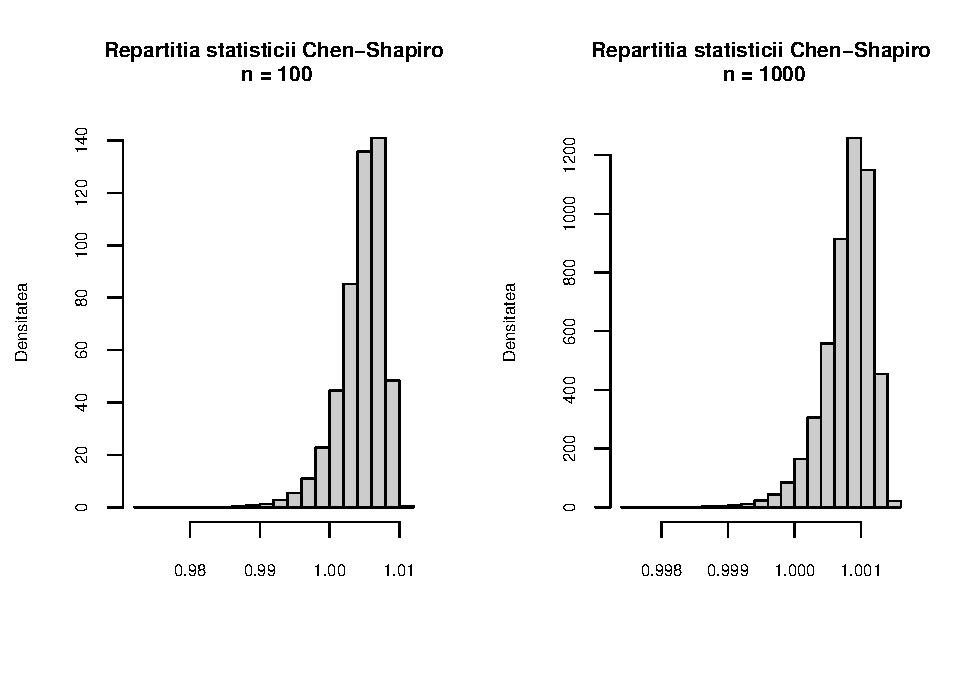
\includegraphics[width=0.8\linewidth]{Lab_4_files/figure-latex/unnamed-chunk-27-1} \end{center}

\subsection{Testul lui Kolmogorov-Smirnov și varianta lui
Lilliefors}\label{testul-lui-kolmogorov-smirnov-si-varianta-lui-lilliefors}

Unul dintre cele mai cunoscute teste (chiar dacă nu cel mai bun) pentru
verificarea ipotezei de normalitate este testul lui Kolmogorov-Smirnov.
Fie \(X_1, X_2, \ldots, X_n\) un eșantion de talie \(n\) dintr-o
populație \(F\) și fie \(\hat{F}_n\) funcția de repartiție empirică
asociată. Testul lui Kolmogorov-Smirnov este folosit pentru a testa dacă
eșantionul provine dintr-o populație specificată \(F^*\) calculând cât
de departe de funcția de repartiție \(F^*\) se află funcția de
repartiție empirică \(\hat{F}_n\).

Ipoteza nulă și ipoteza alternativă a testului sunt date de:

\[
\begin{array}{ll}
  H_0:\, F(x) = F^*(x), \forall x\; \text{(eșantionul provine din $F^*$)}\\
  H_1:\, \exists x \text{ a.i. } F(x) \neq F^*(x) \; \text{(eșantionul nu provine din $F^*$)}
\end{array}
\]

Testul lui Kolmogorov-Smirnov se bazează pe următoarea teoremă (a lui
Kolmogorov-Smirnov):

\begin{rmdinsight}
Fie \((X_n)_n\) un șir de variabile aleatoare independente și indentic
repartizate cu repartiția comună \(\mathbb{P}\circ X^{-1}\) și a cărei
funcție de repartiție \(F\), este continuă. Atunci șirul funcțiilor de
repartiții empirice \((\hat{F}_n)_n\) asociate lui \((X_n)_n\) verifică

\[
  \sqrt{n}\sup_{x\in\mathbb{R}}\left(\hat{F}_n(x) - F(x)\right) \overset{d}{\underset{n\to\infty}{\longrightarrow}} K_1 \quad \text{si} \quad \sqrt{n}\sup_{x\in\mathbb{R}}\left|\hat{F}_n(x) - F(x)\right| \overset{d}{\underset{n\to\infty}{\longrightarrow}} K_2
\]

unde \(K_1\) și \(K_2\) sunt repartiții pe \(\mathbb{R}_+\) numite
repartițiile Kolmogorov-Smirnov și a căror funcție de repartiție sunt,
pentru \(u>0\), date de

\[
  K_1((-\infty, u]) = 1 - e^{-2u^2} \quad \text{si} \quad  K_2((-\infty, u]) = 1+2\sum_{k=1}^{\infty}(-1)^ke^{-2k^2u^2}. 
\]
\end{rmdinsight}

Statistica de test este

\[
  D_n = \sqrt{n}\max_{1\leq i\leq n}\left|\hat{F}_n(x_{(i)}) - F(x_{(i)})\right|.
\]

În cazul ipotezei de normalitate avem
\(F(\cdot) = \Phi(\cdot, \mu, \sigma^2)\)
(\(\Phi(\cdot, \mu, \sigma^2)\) este funcția de repartiție a
\(\mathcal{N}(\mu, \sigma^2)\)) iar \(D_n\) se scrie (ținem cont că
\(\hat{F}_n(x_{(i)}) = \frac{i}{n}\) și evităm mărginirea)

\[
  D_n = \sqrt{n}\max_{1\leq i\leq n}\left\{\Phi(x_{(i)})-\frac{i-1}{n}, \frac{i}{n} - \Phi(x_{(i)})\right\}.
\]

Ipoteza de normalitate este respinsă dacă statistica de test \(D_n\) ia
valori mari. În cazul în care media și varianța sunt necunoscute atunci
(Lilliefors 1967) a propus următoarea variantă a testului
Kolmogorov-Smirnov (Lilliefors)

\[
  D_n' = \sqrt{n}\max_{1\leq i\leq n}\left\{\Phi(x_{(i)}, \bar{x}_n, s_n^2)-\frac{i-1}{n}, \frac{i}{n} - \Phi(x_{(i)}, \bar{x}_n, s_n^2)\right\}.
\]

În R testul Kolmogorov-Smirnov poate fi aplicat apelând funcția
\texttt{ks.test()}. Pentru varianta lui Lilliefors, pachetul
\texttt{nortest} propune funcția \texttt{lillie.test()}.

\begin{Shaded}
\begin{Highlighting}[]
\KeywordTok{library}\NormalTok{(nortest)}

\NormalTok{Attaching package}\OperatorTok{:}\StringTok{ 'nortest'}
\NormalTok{The following object is masked _by_ }\StringTok{'.GlobalEnv'}\OperatorTok{:}

\StringTok{    }\NormalTok{sf.test}

\CommentTok{# esantion normal repartizat }
\NormalTok{x =}\StringTok{ }\KeywordTok{rnorm}\NormalTok{(}\DecValTok{100}\NormalTok{, }\DecValTok{5}\NormalTok{, }\DecValTok{2}\NormalTok{)}
\KeywordTok{ks.test}\NormalTok{(x, }\StringTok{"pnorm"}\NormalTok{, }\DataTypeTok{mean =} \DecValTok{5}\NormalTok{, }\DataTypeTok{sd =} \DecValTok{2}\NormalTok{)}

\NormalTok{    One}\OperatorTok{-}\NormalTok{sample Kolmogorov}\OperatorTok{-}\NormalTok{Smirnov test}

\NormalTok{data}\OperatorTok{:}\StringTok{  }\NormalTok{x}
\NormalTok{D =}\StringTok{ }\FloatTok{0.076928}\NormalTok{, p}\OperatorTok{-}\NormalTok{value =}\StringTok{ }\FloatTok{0.5948}
\NormalTok{alternative hypothesis}\OperatorTok{:}\StringTok{ }\NormalTok{two}\OperatorTok{-}\NormalTok{sided}
\KeywordTok{lillie.test}\NormalTok{(x)}

    \KeywordTok{Lilliefors}\NormalTok{ (Kolmogorov}\OperatorTok{-}\NormalTok{Smirnov) normality test}

\NormalTok{data}\OperatorTok{:}\StringTok{  }\NormalTok{x}
\NormalTok{D =}\StringTok{ }\FloatTok{0.059924}\NormalTok{, p}\OperatorTok{-}\NormalTok{value =}\StringTok{ }\FloatTok{0.5069}

\CommentTok{# esantion repartizat t-student}
\NormalTok{xt =}\StringTok{ }\KeywordTok{rt}\NormalTok{(}\DecValTok{100}\NormalTok{, }\DataTypeTok{df =} \DecValTok{2}\NormalTok{)}
\KeywordTok{ks.test}\NormalTok{(xt, }\StringTok{"pnorm"}\NormalTok{)}

\NormalTok{    One}\OperatorTok{-}\NormalTok{sample Kolmogorov}\OperatorTok{-}\NormalTok{Smirnov test}

\NormalTok{data}\OperatorTok{:}\StringTok{  }\NormalTok{xt}
\NormalTok{D =}\StringTok{ }\FloatTok{0.088898}\NormalTok{, p}\OperatorTok{-}\NormalTok{value =}\StringTok{ }\FloatTok{0.4081}
\NormalTok{alternative hypothesis}\OperatorTok{:}\StringTok{ }\NormalTok{two}\OperatorTok{-}\NormalTok{sided}
\KeywordTok{lillie.test}\NormalTok{(xt)}

    \KeywordTok{Lilliefors}\NormalTok{ (Kolmogorov}\OperatorTok{-}\NormalTok{Smirnov) normality test}

\NormalTok{data}\OperatorTok{:}\StringTok{  }\NormalTok{xt}
\NormalTok{D =}\StringTok{ }\FloatTok{0.25686}\NormalTok{, p}\OperatorTok{-}\NormalTok{value }\OperatorTok{<}\StringTok{ }\FloatTok{2.2e-16}
\end{Highlighting}
\end{Shaded}

Trebuie observat că testul lui Kolmogorov-Smirnov poate fi folosit și
pentru a testa dacă două eșantioane provin din aceeași populație. Fie
\(X_1, X_2, \ldots, X_n\) un eșantion de talie \(n\) dintr-o populație
\(F\) și \(Y1, Y_2, \ldots, Y_m\) un eșantion de talie \(m\) dintr-o
populație \(G\) și vrem să testăm

\[
  H_0: F = G \quad vs\quad H_1: F\neq G
\]

Dacă \(\hat{F}_n\) și respectiv \(\hat{G}_m\) sunt funcțiile de
repartiție empirice asociate celor două eșantioane atunci statistica

\[
  D_{nm} = \sqrt{\frac{nm}{n+m}}\sup_{x\in\mathbb{R}}\left|\hat{F}_n(x) - \hat{G}_m(x)\right|
\]

verifică rezultatul teoremei lui Kolmogorov-Smirnov și putem folosi
această statistică pentru a testa ipotezele \(H_0\,\, vs\,\, H_1\).

Funcția \texttt{ks.test()} permite și compararea a două eșantioane:

\begin{Shaded}
\begin{Highlighting}[]
\CommentTok{# datele provin din aceeasi populatie}
\NormalTok{x =}\StringTok{ }\KeywordTok{rnorm}\NormalTok{(}\DecValTok{150}\NormalTok{, }\DecValTok{10}\NormalTok{, }\DecValTok{1}\NormalTok{)}
\NormalTok{y =}\StringTok{ }\KeywordTok{rnorm}\NormalTok{(}\DecValTok{200}\NormalTok{, }\DecValTok{10}\NormalTok{, }\DecValTok{1}\NormalTok{)}

\KeywordTok{ks.test}\NormalTok{(x, y)}

\NormalTok{    Two}\OperatorTok{-}\NormalTok{sample Kolmogorov}\OperatorTok{-}\NormalTok{Smirnov test}

\NormalTok{data}\OperatorTok{:}\StringTok{  }\NormalTok{x and y}
\NormalTok{D =}\StringTok{ }\FloatTok{0.071667}\NormalTok{, p}\OperatorTok{-}\NormalTok{value =}\StringTok{ }\FloatTok{0.7708}
\NormalTok{alternative hypothesis}\OperatorTok{:}\StringTok{ }\NormalTok{two}\OperatorTok{-}\NormalTok{sided}

\CommentTok{# datele nu provin din aceeasi populatie}
\NormalTok{xt =}\StringTok{ }\KeywordTok{rnorm}\NormalTok{(}\DecValTok{1500}\NormalTok{, }\DecValTok{0}\NormalTok{, }\DecValTok{2}\NormalTok{)}
\NormalTok{yt =}\StringTok{ }\KeywordTok{rt}\NormalTok{(}\DecValTok{2000}\NormalTok{, }\DataTypeTok{df =} \DecValTok{4}\NormalTok{)}

\KeywordTok{ks.test}\NormalTok{(xt, yt)}

\NormalTok{    Two}\OperatorTok{-}\NormalTok{sample Kolmogorov}\OperatorTok{-}\NormalTok{Smirnov test}

\NormalTok{data}\OperatorTok{:}\StringTok{  }\NormalTok{xt and yt}
\NormalTok{D =}\StringTok{ }\FloatTok{0.14267}\NormalTok{, p}\OperatorTok{-}\NormalTok{value =}\StringTok{ }\FloatTok{1.443e-15}
\NormalTok{alternative hypothesis}\OperatorTok{:}\StringTok{ }\NormalTok{two}\OperatorTok{-}\NormalTok{sided}
\end{Highlighting}
\end{Shaded}

\subsection{Studiu comparativ de
putere}\label{studiu-comparativ-de-putere}

În cele ce urmează vom compara puterea testelor Jarque-Bera,
Shapiro-Wilk, Shapiro-Francia și Lilliefors pentru diverse alternative:

\begin{Shaded}
\begin{Highlighting}[]
\KeywordTok{library}\NormalTok{(nortest)}

\NormalTok{ simfun_tests =}\StringTok{ }\ControlFlowTok{function}\NormalTok{(}\DataTypeTok{fun =} \ControlFlowTok{function}\NormalTok{(n) }\KeywordTok{rnorm}\NormalTok{(n), }\DataTypeTok{n =} \DecValTok{250}\NormalTok{) \{}
\NormalTok{   x =}\StringTok{ }\KeywordTok{fun}\NormalTok{(n)}
   \KeywordTok{c}\NormalTok{(}\DataTypeTok{jb =} \KeywordTok{JBtest}\NormalTok{(x)}\OperatorTok{$}\NormalTok{p.value,}
     \DataTypeTok{sw =} \KeywordTok{shapiro.test}\NormalTok{(x)}\OperatorTok{$}\NormalTok{p.value, }
     \DataTypeTok{sf =} \KeywordTok{sf.test}\NormalTok{(x)}\OperatorTok{$}\NormalTok{p.value,  }
     \DataTypeTok{lillie=}\KeywordTok{lillie.test}\NormalTok{(x)}\OperatorTok{$}\NormalTok{p.value)}
\NormalTok{ \}}
 
\end{Highlighting}
\end{Shaded}

\begin{itemize}
\tightlist
\item
  în cazul în care eșantionul provine dintr-o repartiție cu coadă lungă
  (t-student cu 3 grade de libertate):
\end{itemize}

\begin{Shaded}
\begin{Highlighting}[]
\NormalTok{## repartitie cu coada lunga, t(3)}
\NormalTok{rt3 =}\StringTok{ }\ControlFlowTok{function}\NormalTok{(n) }\KeywordTok{rt}\NormalTok{(n, }\DataTypeTok{df=}\DecValTok{3}\NormalTok{)}
\NormalTok{out_rt3 =}\StringTok{ }\KeywordTok{replicate}\NormalTok{(}\DecValTok{10000}\NormalTok{, }\KeywordTok{simfun_tests}\NormalTok{(}\DataTypeTok{fun =}\NormalTok{ rt3, }\DataTypeTok{n =} \DecValTok{75}\NormalTok{))}

\KeywordTok{round}\NormalTok{(}\KeywordTok{apply}\NormalTok{(out_rt3, }\DecValTok{1}\NormalTok{, }\ControlFlowTok{function}\NormalTok{(x) }\KeywordTok{mean}\NormalTok{(x}\OperatorTok{<=}\FloatTok{0.05}\NormalTok{, }\DataTypeTok{na.rm=}\OtherTok{TRUE}\NormalTok{)), }\DecValTok{3}\NormalTok{)}
\end{Highlighting}
\end{Shaded}

\rowcolors{2}{gray!6}{white}

\begin{longtable}{rrrr}
\hiderowcolors
\toprule
Jarque-Bera & Shapiro-Wilk & Shapiro-Francia & Lilliefors\\
\midrule
\endfirsthead
\multicolumn{4}{@{}l}{\textit{(continued)}}\\
\toprule
Jarque-Bera & Shapiro-Wilk & Shapiro-Francia & Lilliefors\\
\midrule
\endhead
\
\endfoot
\bottomrule
\endlastfoot
\showrowcolors
0.807 & 0.78 & 0.827 & 0.622\\*
\end{longtable}

\rowcolors{2}{white}{white}

\begin{itemize}
\tightlist
\item
  în cazul în care eșantionul provine dintr-o repartiție cu coadă scurtă
  (uniormă pe \(\mathcal{U}[0,1]\)):
\end{itemize}

\begin{Shaded}
\begin{Highlighting}[]
\NormalTok{## repartitie cu coada scurta, uniform}
\NormalTok{u =}\StringTok{ }\ControlFlowTok{function}\NormalTok{(n) }\KeywordTok{runif}\NormalTok{(n)}

\NormalTok{out_u =}\StringTok{ }\KeywordTok{replicate}\NormalTok{(}\DecValTok{10000}\NormalTok{, }\KeywordTok{simfun_tests}\NormalTok{(}\DataTypeTok{fun =}\NormalTok{ u, }\DataTypeTok{n =} \DecValTok{65}\NormalTok{))}

\KeywordTok{round}\NormalTok{(}\KeywordTok{apply}\NormalTok{(out_u, }\DecValTok{1}\NormalTok{, }\ControlFlowTok{function}\NormalTok{(x) }\KeywordTok{mean}\NormalTok{(x}\OperatorTok{<=}\FloatTok{0.05}\NormalTok{, }\DataTypeTok{na.rm=}\OtherTok{TRUE}\NormalTok{)), }\DecValTok{3}\NormalTok{)}
\end{Highlighting}
\end{Shaded}

\rowcolors{2}{gray!6}{white}

\begin{longtable}{rrrr}
\hiderowcolors
\toprule
Jarque-Bera & Shapiro-Wilk & Shapiro-Francia & Lilliefors\\
\midrule
\endfirsthead
\multicolumn{4}{@{}l}{\textit{(continued)}}\\
\toprule
Jarque-Bera & Shapiro-Wilk & Shapiro-Francia & Lilliefors\\
\midrule
\endhead
\
\endfoot
\bottomrule
\endlastfoot
\showrowcolors
0.014 & 0.904 & 0.712 & 0.366\\*
\end{longtable}

\rowcolors{2}{white}{white}

\begin{itemize}
\tightlist
\item
  în cazul în care eșantionul provine dintr-o repartiție asimetrică
  (gama \(\Gamma(2,2)\)):
\end{itemize}

\begin{Shaded}
\begin{Highlighting}[]
\NormalTok{## repartitie asimetrica gamma(2,2)}
\NormalTok{g22 =}\StringTok{ }\ControlFlowTok{function}\NormalTok{(n) }\KeywordTok{rgamma}\NormalTok{(n,}\DecValTok{2}\NormalTok{,}\DecValTok{2}\NormalTok{)}

\NormalTok{out_g22 <-}\StringTok{ }\KeywordTok{replicate}\NormalTok{(}\DecValTok{10000}\NormalTok{, }\KeywordTok{simfun_tests}\NormalTok{(}\DataTypeTok{fun =}\NormalTok{ g22, }\DataTypeTok{n =} \DecValTok{50}\NormalTok{))}

\KeywordTok{round}\NormalTok{(}\KeywordTok{apply}\NormalTok{(out_g22, }\DecValTok{1}\NormalTok{, }\ControlFlowTok{function}\NormalTok{(x) }\KeywordTok{mean}\NormalTok{(x}\OperatorTok{<=}\FloatTok{0.05}\NormalTok{, }\DataTypeTok{na.rm=}\OtherTok{TRUE}\NormalTok{)), }\DecValTok{3}\NormalTok{)}
\end{Highlighting}
\end{Shaded}

\rowcolors{2}{gray!6}{white}

\begin{longtable}{rrrr}
\hiderowcolors
\toprule
Jarque-Bera & Shapiro-Wilk & Shapiro-Francia & Lilliefors\\
\midrule
\endfirsthead
\multicolumn{4}{@{}l}{\textit{(continued)}}\\
\toprule
Jarque-Bera & Shapiro-Wilk & Shapiro-Francia & Lilliefors\\
\midrule
\endhead
\
\endfoot
\bottomrule
\endlastfoot
\showrowcolors
0.768 & 0.949 & 0.926 & 0.698\\*
\end{longtable}

\rowcolors{2}{white}{white}

\section*{Referințe}\label{referinte}
\addcontentsline{toc}{section}{Referințe}

\hypertarget{refs}{}
\hypertarget{ref-ChenShapiro1995}{}
Chen, Samuel S., Ling.; Shapiro. 1995. ``An Alernative Test for
Normality Based on Normalized Spacings.'' \emph{Journal of Statistical
Computation and Simulation} 53: 269--87.
doi:\href{https://doi.org/10.1080/00949659508811711}{10.1080/00949659508811711}.

\hypertarget{ref-Joanes1998}{}
Gill, D. N. Joanes; C. A. 1998. ``Comparing Measures of Sample Skewness
and Kurtosis.'' \emph{Journal of the Royal Statistical Society: Series D
(the Statistician)} 47: 183--89.
doi:\href{https://doi.org/10.1111/1467-9884.00122}{10.1111/1467-9884.00122}.

\hypertarget{ref-JarqueBera1987}{}
Jarque, C. M., and A. K. Bera. 1987. ``A Test for Normality of
Observations and Regression Residuals.'' \emph{International Statistical
Review} 55: 163--72.

\hypertarget{ref-Lilliefors1967}{}
Lilliefors, Hubert W. 1967. ``On the Kolmogorov-Smirnov Test for
Normality with Mean and Variance Unknown.'' \emph{Journal of the
American Statistical Association} 62: 399--402.
doi:\href{https://doi.org/10.1080/01621459.1967.10482916}{10.1080/01621459.1967.10482916}.

\hypertarget{ref-Romao2010}{}
Romão, Raimundo; Costa, Xavier; Delgado. 2010. ``An Empirical Power
Comparison of Univariate Goodness-of-Fit Tests for Normality.''
\emph{Journal of Statistical Computation and Simulation} 80: 545--91.
doi:\href{https://doi.org/10.1080/00949650902740824}{10.1080/00949650902740824}.

\hypertarget{ref-RoystonSF1993}{}
Royston, Patrick. 1993. ``A Pocket-Calculator Algorithm for the
Shapiro-Francia Test for Non-Normality: An Application to Medicine.''
\emph{Statistics in Medicine} 12: 181--84.
doi:\href{https://doi.org/10.1002/sim.4780120209}{10.1002/sim.4780120209}.

\hypertarget{ref-ShapiroFrancia1972}{}
Shapiro, R. S., S. S.; Francia. 1972. ``An Approximate Analysis of
Variance Test for Normality.'' \emph{Journal of the American Statistical
Association} 67: 215--16.
doi:\href{https://doi.org/10.1080/01621459.1972.10481232}{10.1080/01621459.1972.10481232}.

\hypertarget{ref-ShapiroWilk1965}{}
Shapiro, S. S., and M. B. Wilk. 1965. ``An Analysis of Variance Test for
Normality (Complete Samples).'' \emph{Biometrika} 52: 591--611.
doi:\href{https://doi.org/10.1093/biomet/52.3-4.591}{10.1093/biomet/52.3-4.591}.

\hypertarget{ref-Thode2002}{}
Thode, Henry C. 2002. \emph{Testing for Normality}. STATISTICS:
Textbooks and Monographs. MARCEL DEKKER, INC.

\hypertarget{ref-Wilk1968}{}
Wilk, M. B., and R. Gnanadesikan. 1968. ``Probability Plotting Methods
for the Analysis of Data.'' \emph{Biometrika} 55: 1--17.
doi:\href{https://doi.org/10.2307/2334448}{10.2307/2334448}.


\end{document}
